\documentclass[sigconf, nonacm]{acmart}

%%% do not modify the following VLDB block %%%
%%% VLDB block start %%%
\usepackage{pvldb}
%%% VLDB block end %%%

\renewcommand\vldbdoi{XX.XX/XXX.XX}
\renewcommand\vldbpages{XXX-XXX}
\renewcommand\vldbavailabilityurl{}

\usepackage[linesnumbered,ruled,vlined]{algorithm2e}
\usepackage{amsmath,amsfonts}
\usepackage{algorithmic}
\usepackage{enumitem}

\usepackage{tikz}
\usetikzlibrary{arrows.meta,decorations.pathreplacing}
\usepackage{pgfplots}
\usepgfplotslibrary{statistics}
\usepackage{xcolor}
\usepackage{colortbl}
\definecolor{bestgreen}{HTML}{DCEFE2}
\definecolor{midyellow}{HTML}{FFF1BF}
\definecolor{accentblue}{HTML}{DCEAF7}
\definecolor{accentred}{HTML}{F6D7DB}
\pgfplotsset{compat=1.17}
\usepackage{amsthm}
\usepackage{multirow}
\usepackage{subcaption}
\usepackage{placeins}
\newtheorem{problem}{Problem}

\newtheorem{definition}{Definition}
\newtheorem{example}{Example}
\newtheorem{observation}{Observation}[section] 
\newtheorem{corollary}{Corollary }[section]
\newtheorem{theorem}{Theorem}[section]
\newtheorem{lemma}{Lemma}[section]
\newtheorem{property}{Property}[section]
%\newenvironment{proof}{ {\it  Proof:} }{\hfill $\square$\par}  


\newcommand{\kw}[1]{{\ensuremath {\mathsf{#1}}}\xspace}
\newcommand{\kwnospace}[1]{{\ensuremath {\mathsf{#1}}}}
\newcommand{\stitleunderline}[1]{\vspace{0.7ex}\noindent\underline{{\bf #1}}}
%\newcommand{\stitleunderline}[1]{\vspace{1ex} \noindent{\bf #1}}
\newcommand{\stitle}[1]{\vspace{0.7ex} \noindent{\bf #1}}
\long\def\comment#1{}
\newcommand{\eop}{\hspace*{\fill}\mbox{$\Box$}}
\newcommand{\eopfill}{\hfill{\rule[0pt]{1.3ex}{1.3ex}}}
\def\done{\hspace*{\fill}$\square$\par}

%% ---------------------------------------------------------------
%% Unified notation macros (single source of truth)
%%
%%   \avgsim(C)   闂?average pairwise similarity of clique C
%%                  = (2 / |C|(|C|-1)) * sum_{u<v in C} sim(u,v)
%%
%%   \simsum(C)   闂?total pairwise similarity sum of clique C
%%                  = sum_{u<v in C} sim(u,v)
%%
%%   \W(C)        闂?semantic surplus of clique C w.r.t. threshold tau
%%                  = simsum(C) - tau * C(|C|,2)  (positive iff avgsim >= tau)
%%
%%   \acc[v]      闂?accumulated similarity of candidate v to current clique C
%%                  = sum_{u in C} sim(u,v)
%%
%%                  = avgsim(C) * C(|C|+1,2) - simsum(C)
%% ---------------------------------------------------------------
\newcommand{\StructBK}{\textsc{Struct\-BK}}
\newcommand{\semBK}{\textsc{SemBK}}
\newcommand{\subEnum}{\textsc{StrSub}}
\newcommand{\monoSemMCE}{\textsc{Mono\-Sem\-MCE}}
\newcommand{\pairSim}{\textsc{PairSim-MCE}}
\newcommand{\avgsim}{\mathrm{avgSim}}
\newcommand{\simsum}{\mathit{simSum}}
\newcommand{\W}{\mathit{W}}
\newcommand{\acc}{\mathit{acc}}


\begin{document}
\title{Maximal Semantic Clique Enumeration in Vector-Attributed Graphs}
%%
%% The "author" command and its associated commands are used to define the authors and their affiliations.
\author{Tianyi Gao}
\affiliation{%
  \institution{Beijing Institute of Technology}
  \city{Beijing}
  \country{China}
}
\email{tygao\_bit@163.com}

\author{Hongchao Qin}
\affiliation{%
  \institution{Beijing Institute of Technology}
  \city{Beijing}
  \country{China}
}
\email{qhc\_neu@gmail.com}

%%
%% The abstract is a short summary of the work to be presented in the
%% article.
\begin{abstract}
Maximal clique enumeration is a fundamental primitive for graph analysis, yet structural completeness alone cannot identify semantically coherent groups in vector-attributed graphs.  Adding a collective similarity constraint makes the problem substantially harder: average pairwise similarity is non-monotone over the subset lattice, so the pivot invariant behind scalable structural enumeration no longer holds.  We formalize maximal semantic clique (MSC) enumeration under inclusion-wise maximality and develop two exact algorithms.  \subEnum\ restores structural pivoting by separating structural MCE from bounded semantic subset enumeration.  \monoSemMCE\ targets selective thresholds through a canonical-parent theorem: deleting a minimum-contribution vertex from any feasible clique yields a unique feasible parent.  The resulting reverse search generates each feasible state once without visited tables or materialized size layers.  Across eight datasets and a fixed similarity-quantile grid, the two methods complete all 24 workloads, while the exact \semBK\ baseline reaches the 1,200-second limit on 15.  At $q_{99}$, \monoSemMCE\ is $2.92\times$--$6.24\times$ faster than \subEnum.  Output-family analysis further shows Extended B$^3$ Recall of 0.156 and 0.544 for pairwise-threshold clique mining on two real graphs, quantifying its fragmentation of collectively feasible complete groups.
\end{abstract}
\maketitle

%%% do not modify the following VLDB block %%
%%% VLDB block start %%%
\vldbtopmatter
%%% VLDB block end %%%

\section{Introduction}
\label{sec:intro}

Graphs with rich vertex attributes are ubiquitous in modern data management and analytics. Social networks associate users with profile embeddings, knowledge graphs attach entity descriptions to nodes, and biological networks annotate proteins with functional vectors. In all these settings, the attribute space carries semantic meaning that is largely orthogonal to the topological structure: two vertices may be structurally adjacent yet semantically distant, and vice versa. Identifying cohesive subgraphs that are simultaneously structurally dense and semantically coherent is therefore a recurring need across domains.

The maximal clique is a classic structural model of cohesion: every pair of vertices is connected, guaranteeing the highest possible edge density. However, in vector-attributed graphs, a clique may group vertices that are heterogeneous in the attribute space. Conversely, attribute-based community detection methods (e.g., modularity optimization with attribute homogeneity) often sacrifice structural guarantees and produce loosely connected groups. This tension motivates a joint model that enforces both structural completeness and semantic coherence.

\stitle{The MSC Problem.}
We study the problem of enumerating \emph{maximal semantic cliques} (MSCs) in a vector-attributed graph. Each vertex carries a real-valued attribute vector; pairwise semantic similarity is measured by cosine similarity. Given a threshold $\tau$, a clique is a $\tau$-semantic clique if its average pairwise similarity is at least $\tau$. An MSC is an inclusion-wise maximal $\tau$-semantic clique: no strict superset is also a $\tau$-semantic clique. The task is to enumerate \emph{all} MSCs of the input graph.

This formulation has two salient features. First, the average constraint is a \emph{global} property of the clique: it depends on all $\binom{|C|}{2}$ pairwise similarities, not on any single edge. This makes it fundamentally different from edge-level semantic constraints (e.g., requiring every edge to exceed a threshold), which are local and monotone. Second, the average is non-monotone over the subset lattice: adding a vertex can raise or lower the average, so a partial clique that currently violates the constraint may still grow into a valid MSC, while one that satisfies it may admit no feasible extension. This non-monotonicity invalidates the structural invariants that underpin the efficiency of classical maximal clique enumeration (MCE) algorithms.

\stitle{Why Classical MCE Does Not Suffice.}
The Bron--Kerbosch (BK) algorithm and its modern variants achieve state-of-the-art performance for MCE through two key techniques: \emph{pivot-based pruning} (Tomita et al.) and \emph{degeneracy ordering} (Eppstein et al.). Pivot pruning relies on the fact that structural maximality is closed under supersets: if a vertex $u$ is adjacent to the current pivot $p$, any maximal clique containing $u$ also contains $p$, so $u$ can be safely suppressed as an expansion root. Under the average constraint, this closure breaks: a clique containing $u$ but not $p$ may satisfy $\avgsim \geq \tau$ while $\{p,u\}$ does not. Consequently, pivoting is not merely ineffective---it is \emph{incorrect} for MSC enumeration. A direct BK adaptation must therefore forgo pivoting entirely and defer all semantic evaluation to the leaves, degenerating to exhaustive structural enumeration regardless of $\tau$.

\stitleunderline{Problem formulation.}
We formalize maximal semantic clique enumeration under an inclusion-wise
maximal average-similarity constraint, establish its computational hardness,
and identify the non-monotonicity that prevents direct use of structural BK
pivoting.

\stitleunderline{Exact enumeration algorithms.}
We develop \subEnum, which separates structural MCE from bounded semantic
subset enumeration, and \monoSemMCE, whose canonical-parent relation organizes
high-threshold search without visited tables or materialized size layers. Both
algorithms preserve the complete MSC output set.

\stitleunderline{Large-scale evaluation.}
We evaluate exactness, runtime, memory, scalability, pruning mechanisms, and
output semantics on eight vector-attributed graphs under a fixed
similarity-quantile protocol. The results identify the operating regions of
the two search organizations and quantify their gains over the exact semantic
baseline.
\stitle{Paper Organization.}
Section~\ref{sec:pre} formalizes the problem and establishes hardness. Section~\ref{sec:framework} presents the baseline \semBK\ algorithm and explains why pivoting fails. Section~\ref{sec:algorithms} develops \subEnum\ and \monoSemMCE. Section~\ref{sec:opt} describes shared implementation optimizations. Section~\ref{sec:exp} reports experimental results. Section~\ref{sec:related} discusses related work, and Section~\ref{sec:conclusion} concludes.
\section{Preliminaries}
\label{sec:pre}

\subsection{Notations and Problem Definition}

We study a \emph{vector-attributed graph} $\mathcal{G}=(V,E,\mathbf{X})$,
where $V$ is the vertex set, $E \subseteq \binom{V}{2}$ is the edge set,
and $\mathbf{X}=\{\mathbf{x}_v \in \mathbb{R}^D \mid v \in V\}$ assigns a
$D$-dimensional attribute vector to each vertex.

\begin{definition}[Similarity Function]
  A similarity function $\mathrm{sim}: \mathbb{R}^D \times \mathbb{R}^D \rightarrow [-1,1]$
  is a symmetric, bounded function measuring the semantic closeness of two
  attribute vectors.  We assume all attribute vectors are $\ell_2$-normalized,
  so that $\mathrm{sim}$ coincides with cosine similarity and its range is
  naturally $[-1,1]$.
\end{definition}

Throughout this paper we work with normalized vectors and precompute
$\mathrm{sim}(u,v)$ for all $(u,v)\in E$.  The threshold $\tau \in [-1,1]$
is drawn from the same range.

\begin{definition}[Clique]
  A set $C \subseteq V$ is a \emph{clique} in $\mathcal{G}$ if every pair of distinct
  vertices in $C$ is connected by an edge, i.e., $\{u,v\} \in E$ for all $u \neq v \in C$.
\end{definition}

Classical maximal clique enumeration (MCE) seeks cliques that cannot be extended by
any additional vertex while preserving the clique property.  In vector-attributed graphs,
however, structural density alone is insufficient to characterize semantically coherent
groups: a clique may consist of vertices that are structurally adjacent yet semantically
heterogeneous.  To capture both aspects jointly, we introduce two companion quantities.

\begin{definition}[Pairwise Similarity Sum and Average Pairwise Similarity]
  For a clique $C$ of size $k = |C| \geq 2$, the \emph{pairwise similarity sum} is
  \[
    \simsum(C) = \sum_{\{u,v\}\subseteq C}\mathrm{sim}(u,v),
  \]
  and the \emph{average pairwise similarity} is
  \[
    \avgsim(C) = \frac{\simsum(C)}{\tbinom{k}{2}}.
  \]
\end{definition}

\begin{definition}[Semantic Clique]
  Given a threshold $\tau \in [-1,1]$, a clique $C$ with $|C|\geq2$ is a
  \emph{$\tau$-semantic clique} if $\avgsim(C) \geq \tau$.
\end{definition}

For algorithmic purposes, we equivalently track the
\emph{semantic surplus}
\[
  \W(C) = \simsum(C) - \tau\tbinom{k}{2},
\]
which is non-negative if and only if $\avgsim(C) \geq \tau$.  Working with $\simsum$
and $\W$ avoids division at every recursive step; $\avgsim$ is used only when a
human-readable quantity is required.

\begin{definition}[MSC]
  \label{def:msc}
  Given $\mathcal{G}=(V,E,\mathbf{X})$ and threshold $\tau \in [-1,1]$, a
  $\tau$-semantic clique $C \subseteq V$ is a \emph{maximal semantic clique}
  (MSC) if there is no $\tau$-semantic clique $C' \supsetneq C$.
\end{definition}

This is inclusion-wise maximality, not merely the absence of a feasible
single-vertex extension.  The distinction matters because average feasibility
is non-monotone.  For example, let $\tau=0.6$ and let four vertices form a
clique with $\mathrm{sim}(a,b)=0.6$,
$\mathrm{sim}(a,u)=\mathrm{sim}(b,u)=\mathrm{sim}(a,v)=
\mathrm{sim}(b,v)=0.5$, and $\mathrm{sim}(u,v)=1$.  The feasible clique
$\{a,b\}$ has no feasible single-vertex extension, since either three-vertex
average is $1.6/3<0.6$, but the strict superset $\{a,b,u,v\}$ is feasible
with average $3.6/6=0.6$.  Consequently, algorithms may use the absence of a
feasible single extension only to generate candidates; a global containment
test is still required for MSC output.

\begin{figure}[!htb]
  \centering
  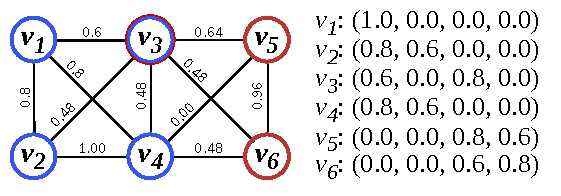
\includegraphics[width=0.8\linewidth,page=1]{fig/pictures.pdf}
  \caption{Running example with vector attributes and edge similarities.}
  \Description{Two overlapping four-vertex cliques with six vector-labeled vertices and pairwise similarity labels.}
  \label{fig:example}
\end{figure}

\begin{example}
  \label{ex:msc}
  Figure~\ref{fig:example} shows a vector-attributed graph with six vertices.
  Edge labels give the precomputed pairwise similarities.
  With threshold $\tau=0.6$, consider the two structural cliques
  \begin{align*}
    M_1&=\{v_1,v_2,v_3,v_4\}, &
    M_2&=\{v_3,v_4,v_5,v_6\}.
  \end{align*}

  Let $C_1=\{v_1,v_2,v_3,v_4\}$, $C_2=\{v_3,v_5,v_6\}$, and
  $C_3=\{v_3,v_4,v_5,v_6\}$. Their total and average similarities are
  \begin{align*}
    \simsum(C_1)&=4.16, & \avgsim(C_1)&\approx0.693\geq\tau,\\
    \simsum(C_2)&=2.08, & \avgsim(C_2)&\approx0.693\geq\tau,\\
    \simsum(C_3)&=2.56, & \avgsim(C_3)&\approx0.427<\tau.
  \end{align*}
  Thus $C_1$ and $C_2$ are $\tau$-semantic cliques, whereas the structurally valid
  clique $C_3$ is not.

  Moreover, neither $C_1$ nor $C_2$ has a strict superset that is a
  $\tau$-semantic clique, so both are MSCs.
\end{example}

\stitle{Problem Statement.}
\begin{problem}[MSC Enumeration]
Given a vector-attributed graph $\mathcal{G}=(V,E,\mathbf{X})$ and a threshold
$\tau \in [-1,1]$, enumerate all MSCs of $\mathcal{G}$.
\end{problem}


\subsection{Challenges}
\label{sec:challenges}
\stitle{Hardness.}
MSC enumeration contains classical MCE as a special case.  When singleton
outputs are excluded and $\tau$ does not exceed the minimum similarity on any
edge, every structural maximal clique of size at least two satisfies the
semantic constraint, so the $\Omega(3^{n/3})$ output lower bound carries over.
The associated decision problem is NP-complete.
\begin{theorem}
  \label{thm:np-complete}
Given $\mathcal{G}=(V,E,\mathbf{X})$, threshold $\tau\in[-1,1]$, and integer $k$,
  deciding whether an MSC of size $\geq k$ exists is \emph{NP-complete}.
\end{theorem}
\begin{proof}
  \textit{NP membership.}  The decision instance is positive if and only if
  it contains a $\tau$-semantic clique $C$ of size at least $k$.  The
  forward implication is immediate.  For the reverse implication, the finite
  family of feasible clique supersets of $C$ contains an inclusion-wise
  maximal member, whose size is at least $|C|\geq k$.  A certificate therefore
  need only provide such a feasible clique $C$: verifying all edges and
  $\avgsim(C)\geq\tau$ takes $O(|C|^2)$ time.  It is unnecessary, and under
  the non-monotone constraint insufficient, to verify maximality by checking
  only single-vertex extensions.

  \textit{NP-hardness.}  We reduce from the \textsc{Clique} decision
  problem~\cite{karp1972}, which asks whether $G_0=(V,E)$ contains a
  clique of size $\geq k$.
  Assign $\mathbf{x}_v = \mathbf{e}_1$ to every vertex, so
  $\mathrm{sim}(u,v) = 1$ for every edge, and set $\tau = 1$.
  Under this assignment $\avgsim(C) = 1 \geq \tau$ for every clique $C$,
  so every structural maximal clique is an MSC and vice versa.
  Any clique of size $\geq k$ in $G_0$ is contained in some structural
  maximal clique of size $\geq k$, which is also an MSC of size $\geq k$.
  Conversely, any MSC of size $\geq k$ is a clique of size $\geq k$
  in $G_0$.  Hence a size-$k$ MSC exists if and only if $G_0$ contains
  a clique of size $\geq k$, completing the reduction.
\end{proof}

The output sets of MSC enumeration and MCE are incomparable: a structural
maximal clique with $\avgsim(M)<\tau$ may contain semantically maximal subsets
that MCE never generates, while valid MSCs need not be structurally maximal.
The output size, and hence the computational cost, is $\tau$-dependent in a
non-trivial way that we characterize below.

\stitle{Output Distribution and Practical Scope.}
The number of MSCs and their sizes vary substantially with $\tau$.
At sufficiently low $\tau$, almost every clique satisfies the average constraint and the
output converges toward that of classical MCE.
As $\tau$ increases, large structural cliques that previously satisfied the
constraint cease to do so and are replaced by many smaller semantically
feasible sub-cliques, none of which subsumes another.
This \emph{fragmentation effect} can inflate the output size by orders of
magnitude relative to MCE\@.
At sufficiently high $\tau$, the constraint eliminates most cliques outright
and the output shrinks considerably.

The intermediate fragmentation band carries the largest output volume and is
therefore inherently time-consuming---any correct algorithm must enumerate
all output cliques, so the output size itself imposes a lower bound on
runtime.  Low $\tau$ is appropriate when the goal is to filter out
structurally maximal cliques that are semantically too loose; high $\tau$
is appropriate when the goal is to surface only the most semantically
coherent groups.  The exact $\tau$ values at which these transitions occur
depend on the similarity distribution of the underlying dataset and cannot
be fixed a priori. Section~\ref{sec:exp} therefore evaluates a fixed grid of
per-dataset edge-similarity quantiles rather than choosing absolute thresholds
after observing runtimes.

\stitle{Non-monotonicity and Framework Incompatibility.}
The core difficulty is that $\avgsim$ is non-monotone over the subset lattice.
In classical MCE, structural feasibility is monotone and maximality is enforced
implicitly by the $P=\emptyset$ invariant at every leaf, so the set of feasible
extensions can be characterized solely by the current state of $C$.
Under the average constraint, no such invariant exists: a partial clique with
$\avgsim(C)<\tau$ may still grow into a valid MSC, while one with
$\avgsim(C)\geq\tau$ may admit no feasible extension. Furthermore, whether a
candidate vertex can participate in a valid extension depends on its accumulated
similarity to the current partial clique, which evolves throughout the recursion
and cannot be captured by structural conditions alone. As a result, the pruning mechanisms based on structural monotonicity
lose their foundation, and the pivot strategy no longer applies.
Direct adaptations of BK are therefore forced to defer all semantic
evaluation to the leaves, where $\tau$ appears only in validation
rather than guiding the search itself.


\section{Framework}
\label{sec:framework}
\label{sec:sembk}

\stitle{Framework Overview.}
We derive a baseline search procedure by adapting the Bron--Kerbosch (BK)
recursion to the semantic-clique setting under the average constraint.  The standard
partition $(P,X)$ remains useful for structural enumeration, but the semantic
constraint is defined at the clique level: whether a partial clique can
eventually satisfy the threshold depends on $\avgsim$ over all vertex pairs
within the clique.  As a consequence, the pivoting strategy, which relies on
local structural properties, is no longer directly applicable.  The baseline
therefore retains the BK recursion and degeneracy ordering while excluding
pivoting, and enforces semantic maximality via a secondary \textsc{Check}
pass on $X$ at each leaf.

\begin{algorithm}[t]
  \small
  \caption{Semantic BK with Check}
  \label{alg:semantic-max-clique}
  \SetKwFunction{FSearch}{Search}
  \SetKwProg{Fn}{Function}{:}{}

  \textbf{Input}: $G=(V,E)$, semantic vectors $\{x_v\}$, threshold $\tau$\\
  \textbf{Output}: All maximal semantic cliques $C$ s.t. $\avgsim(C) \geq \tau$

  Precompute $\mathrm{sim}(u,v)$ and degeneracy ordering $\sigma$\;
  \For{each $v \in \sigma$ \textbf{in parallel}}{
    $P \leftarrow \{u \in N(v) \mid \sigma(u) > \sigma(v)\}$\;
    $X \leftarrow \{u \in N(v) \mid \sigma(u) < \sigma(v)\}$\;
    Initialize $\acc[u] \leftarrow \mathrm{sim}(u, v)$ for all $u \in N(v)$\;
    \FSearch{$C=\{v\}, \simsum=0, P, X, \acc, \textit{mode}=\emptyset, 0$}
  }

  \BlankLine
  \Fn{\FSearch{$C, \simsum, P, X, \acc, \textit{mode}, k_{\min}$}}{
    $k \leftarrow |C|,\ \textit{foundLonger} \leftarrow \mathbf{false}$\;
    \For{each $v \in P$}{
      $\simsum' \leftarrow \simsum + \acc[v]$\;
      $P \leftarrow P \setminus \{v\}, P' \leftarrow P \cap N(v), X' \leftarrow X \cap N(v)$\;
      $\acc[u] \gets \acc[u] + \mathrm{sim}(u,v)$ \textbf{for} $u \in P' \cup X'$\;
      $\textit{res} \leftarrow$ \FSearch{$C \cup \{v\}, \simsum', P', X', \acc, \textit{mode}, k_{\min}$}\;
      $\acc[u] \gets \acc[u] - \mathrm{sim}(u,v)$ \textbf{for} $u \in P' \cup X'$\;

      \If{$\textit{res}$}{
        $\textit{foundLonger} \leftarrow \mathbf{true}$\;
        \lIf{$\textit{mode} = \mathrm{CHECK}$}{\Return \textit{true}}
      }
      $X \leftarrow X \cup \{v\}$\;
    }

    \If{$\neg \textit{foundLonger}$}{
      \lIf{$k \geq 2 \land 2 \cdot \simsum / (k(k-1)) < \tau$}{\Return \textit{false}}
      \lIf{$\textit{mode} = \mathrm{CHECK}$}{\Return $k > k_{\min}$}

      \If{$X \neq \emptyset$}{
        \If{\FSearch{$C, \simsum, X, \emptyset, \acc, \mathrm{CHECK}, k$}}{
          \Return \textit{true}\;
        }
      }

      \textbf{output} $C$\;
      \Return \textit{true}\;
    }
    \Return $\textit{foundLonger}$\;
  }
\end{algorithm}

\begin{figure}[!htb]
  \centering
  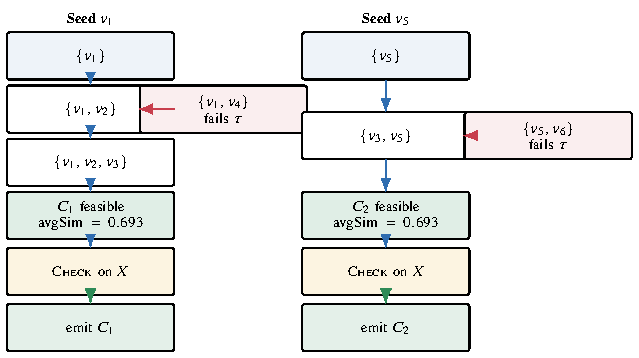
\includegraphics[width=0.92\linewidth]{tex-data/fig/sembk_workflow.pdf}
  \caption{\semBK\ traversal on the running example.}

  \Description{A rooted search tree whose branches follow the example graph's degeneracy order and mark feasible and infeasible leaves.}
  \label{fig:alg1}
\end{figure}

\stitle{[Lines 4--8]: Outer Traversal.}
The outer loop iterates over vertices in degeneracy order $\sigma$.  For a
seed vertex $v$, its later neighbors under $\sigma$ form the candidate set
$P$, and its earlier neighbors are placed in $X$.  This partition guarantees
that every structural maximal clique is generated by exactly one seed,
because the unique vertex of minimum degeneracy index in any clique serves
as its seed and sees all co-members in its $P$.  Since every MSC is contained in at least one structural maximal clique
(as established later in Lemma~\ref{lem:containment}), the same
partition ensures completeness for the semantic problem without
modification.

\stitle{[Lines 9--29]: Recursive Search.}
Within each recursive call, the algorithm explores all vertices in $P$ as
expansion roots.  For each candidate $v$, it updates $\simsum$ and the
auxiliary accumulation array $\acc$, then recurses on the reduced candidate
and exclusion sets $(P', X')$.  When the recursion reaches a leaf
($\textit{foundLonger} = \mathbf{false}$), it first tests the average
constraint: if $\avgsim(C) < \tau$, the branch is pruned immediately.
Otherwise, semantic maximality must be verified: a clique $C$ with
$\avgsim(C) \geq \tau$ and $P = \emptyset$ could still be non-maximal if
some vertex in $X$ can extend it to a larger valid clique.  The algorithm
therefore invokes \textsc{Search} on $X$ in \textsc{Check} mode with
$k_{\min} = |C|$.  In \textsc{Check} mode, the recursion explores
extensions through $X$ and returns \textit{true} as soon as it finds any
valid clique strictly larger than $C$; if no such extension exists, $C$ is
emitted.  The strict size condition $k > k_{\min}$ is necessary because the
\textsc{Check} recursion may reach sub-cliques of $C$ itself; without
recording $k_{\min}$, these would be misidentified as valid extensions.

\stitle{Why pivoting is not used.}
In standard BK, a pivot $p\in P\cup X$ guarantees that each structural maximal
clique in the current branch contains either $p$ or a vertex in
$P\setminus N(p)$.  Hence vertices in $P\cap N(p)$ need not become expansion
roots.  This argument depends on structural feasibility being preserved when
an adjacent pivot is added.

The average constraint invalidates that implication.  Consider a complete
graph on $\{s,p,u,w\}$ at the BK state $C=\{s\}$,
$P=\{p,u,w\}$, and $X=\emptyset$.  Let the three similarities within
$\{s,u,w\}$ equal $0.9$, the three similarities incident to $p$ equal $0$,
and $\tau=0.6$.  Then $\{s,u,w\}$ is an MSC with average $0.9$, whereas its
only strict clique superset has average $0.45$.  Choosing $p$ as the pivot
leaves only $p$ in $P\setminus N(p)$, so every explored child contains $p$
and the valid MSC $\{s,u,w\}$ is lost.  Pivot-free branching is therefore
required for the direct semantic BK baseline.
\stitle{Complexity.}
\begin{theorem}[Time and Space Complexity]
  \label{the:alg1complexity}
  Let $d_G$ be the degeneracy of $G$, let $\mathcal{L}$ be the feasible
  terminal states reached by the outer search, and let $X_C$ be the candidate
  set examined by \textsc{Check} for $C\in\mathcal{L}$.  The running time is
  $O^*(n2^{d_G}+\sum_{C\in\mathcal{L}}2^{|X_C|})$, where $O^*$ suppresses
  polynomial set-intersection costs.  A graph-independent upper bound is
  $O^*(3^n)$.  With $p$ workers, the implementation uses
  $O(m+nD+pn^2)$ worst-case space.
\end{theorem}
\begin{proof}
  A degeneracy seed has at most $d_G$ later neighbors.  Without pivoting, its
  outer recursion may visit every subset of those neighbors, giving
  $O^*(n2^{d_G})$ states.  For a feasible terminal $C$, \textsc{Check} may
  independently visit every subset of $X_C$.  The same earlier extension can
  be reconsidered for several terminals; charging a state to a pair of nested
  vertex sets gives the safe $O^*(3^n)$ bound.  Similarities and sparse
  adjacency require $O(m+nD)$ storage.  Each worker owns an $O(n)$
  accumulator, while decreasing candidate arrays retained by a worst-case
  \textsc{Check} stack total $O(n^2)$.
\end{proof}
\stitle{Design Implication.}
\semBK\ is the direct semantic-search baseline and establishes exact
inclusion-wise maximality through its \textsc{Check} pass. Its pivot-free
branching and repeated extension checks arise from the same property: average
similarity couples all pairs in a clique and cannot be summarized by local
adjacency alone. Section~\ref{sec:algorithms} develops two exact search
organizations that expose additional structural or semantic pruning.


%%-------------------------------------------------------------------
\section{Proposed Algorithms}
\label{sec:algorithms}
This section presents two exact algorithms that exploit the global structure
of the average constraint from different directions.

\subEnum\ (Section~\ref{sec:strsub}) resolves the pivot incompatibility
by decoupling structural and semantic search.  The pivot is applied
without modification to a $\tau$-agnostic structural phase, restoring
the $O(3^{n/3})$ BK guarantee; $\tau$ is then enforced in a subsequent
intra-clique enumeration phase. Complementary sorted-edge and vertex-contribution
upper bounds introduced in Phase~2 skip subset-size layers that cannot satisfy
$\tau$. Its cost is governed by structural MCE and by the sizes of the
resulting host cliques.

\monoSemMCE\ (Section~\ref{sec:monosem-mce}) departs from the BK
framework entirely.  Motivated by the observation that \subEnum, despite
its pruning improvements, still processes all structural maximal cliques
irrespective of their semantic quality, \monoSemMCE\ introduces a
canonical reverse-search strategy in which $\tau$ drives enumeration
from the first expansion step.  A deterministic feasible parent gives
each feasible clique one generation path, while depth-first traversal
avoids storing a complete size layer.  The method is particularly
effective at high $\tau$, where few candidate extensions pass the
surplus test.

Graph size and structural clique growth determine the crossover between the
two methods. We therefore evaluate them on the same quantile grid: \subEnum\
provides broad threshold coverage, while \monoSemMCE\ specializes the search
for selective high-$\tau$ workloads.

%%-------------------------------------------------------------------
\subsection{\subEnum: Structural Decomposition and Subset Enumeration}
\label{sec:strsub}

\stitle{Structural--Semantic Decoupling and Containment.}
The validity of the Bron--Kerbosch pivot rests on a structural invariant:
every structural maximal clique must contain at least one vertex from
$P \setminus N(u)$ for any pivot $u \in P \cup X$.  This invariant is
violated when the average-similarity constraint is incorporated directly
into the branching procedure, because $\avgsim$ is a \emph{global}
property of a candidate set and does not decompose along the local
neighborhood structure used to justify the pivot.  Consequently, the
semantic variant \semBK\ must forgo pivoting entirely, which
undermines the $O(3^{n/3})$ worst-case guarantee of the standard
algorithm~\cite{tomita2006}.

\begin{algorithm}[t]
  \small
  \caption{\subEnum: Structural Decomposition and Subset Enumeration}
  \label{alg:strsub}
  \SetKwFunction{FBK}{BK}
  \SetKwProg{Fn}{Function}{:}{}

  \KwIn{$G=(V,E)$, similarities $\{\mathrm{sim}(u,v)\}_{(u,v)\in E}$, threshold $\tau$}
  \KwOut{All MSCs $\mathcal{R}$}

  $\mathcal{F} \leftarrow \emptyset$\;
  \tcc{Pipelined structural MCE and semantic processing}
  Build degeneracy ordering $\sigma$\;
  \For{each $v \in \sigma$ \textbf{in parallel}}{
    $P \leftarrow \{u \in N(v) \mid \sigma(u) > \sigma(v)\}$\;
    $X \leftarrow \{u \in N(v) \mid \sigma(u) < \sigma(v)\}$\;
    Run $\FBK(\{v\},P,X)$ with the following callback at each leaf $M$\;
  }

  \tcc{Callback: intra-clique semantic enumeration}
  \For{each structural leaf $M$ produced by a worker}{
    \lIf{$\avgsim(M) \geq \tau$}{$\mathcal{F} \leftarrow \mathcal{F} \cup \{M\}$; \textbf{continue}}
    \tcc{Admissible layer bounds}
    Sort edges of $M$ by similarity descending\;
    $k^* \leftarrow \max\!\bigl\{k \in [2,|M|-1] \mid \bar{e}_k \geq \tau\bigr\}$\;
    \lIf{$k^*$ does not exist}{\textbf{continue}}
    $\mathit{lmax} \leftarrow \emptyset$;\quad $\mathit{umask} \leftarrow \mathbf{0}$\;
    \For{$k \leftarrow k^*$ \KwTo $2$}{
      Compute the vertex-contribution bound $\bar{q}_k$ for size $k$\;
      \lIf{$\bar{q}_k < \tau$}{\textbf{continue}}
      \For{each size-$k$ subset $S \subseteq M$}{
        \lIf{$(S \mathbin{\&}\ \mathit{umask}) = S$
          \textbf{ and } $\exists\, T \in \mathit{lmax} : S \subseteq T$}{\textbf{continue}}
        \If{$\avgsim(S) \geq \tau$}{
          $\mathit{lmax} \leftarrow \mathit{lmax} \cup \{S\}$\;
          $\mathit{umask} \leftarrow \mathit{umask} \mid S$\;
          $\mathcal{F} \leftarrow \mathcal{F} \cup \{S\}$\;
        }
      }
    }
  }

  \tcc{Phase 3: Exact global filter}
  Sort $\mathcal{F}$ by $|\cdot|$ descending; remove exact duplicates\;
  Initialize an empty inverted index $\mathit{inv}:v\mapsto\emptyset$\;
  $\mathcal{R} \leftarrow \emptyset$\;
  \For{each equal-size group $\mathcal{G}\subseteq\mathcal{F}$ in descending size}{
    \For{each $S\in\mathcal{G}$ \textbf{in parallel}}{
      $r \leftarrow \displaystyle\mathop{\arg\min}_{v \in S}\ |\mathit{inv}[v]|$\;
      Keep $S$ iff no $T$ referenced by $\mathit{inv}[r]$ satisfies $S\subsetneq T$\;
    }
    Insert every kept $S\in\mathcal{G}$ into $\mathcal{R}$ and $\mathit{inv}$\;
  }
  \Return $\mathcal{R}$\;
\end{algorithm}
Figure~\ref{fig:alg2} separates the two host-clique outcomes. Gray marks
structural or global processing, green marks accepted feasible states, and
amber marks the bounded search triggered by an infeasible host. Thus $M_1$
is accepted as $C_1$, whereas subset enumeration within $M_2$ recovers $C_2$.

\begin{figure}[!htb]
  \centering
  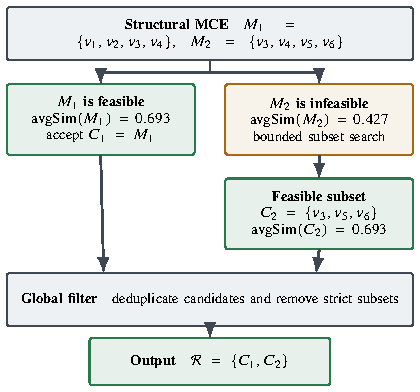
\includegraphics[width=0.8\linewidth]{tex-data/fig/strsub_workflow.pdf}
  \caption{\subEnum\ execution on the running example.}



  \Description{A flow diagram from two structural maximal cliques through direct acceptance or bounded subset enumeration to the final candidate filter.}
  \label{fig:alg2}
\end{figure}


The key insight behind \subEnum\ is that the structural and semantic
layers of the problem can be \emph{decoupled}.  Specifically, the
Tomita pivot can be applied without modification to the purely
structural problem of enumerating maximal cliques in $G$, because that
problem carries no average-similarity constraint.  The threshold $\tau$
is then enforced in a second, independent pass confined to each
structural maximal clique.  The theoretical basis for this decoupling
is the following containment lemma.

\begin{lemma}[Structural Superset of MSCs]
  \label{lem:containment}
  Every MSC is contained in at least one structural maximal clique of $G$.
  That is, for every MSC $C$, there exists a structural maximal clique
  $M$ such that $C \subseteq M$.
\end{lemma}

\begin{proof}
  By definition, every MSC is a clique of $G$.  Let $C$ be an arbitrary
  MSC, and consider the family
  \[
    \mathcal{F} = \{D \subseteq V \mid C \subseteq D \text{ and } D
    \text{ is a clique in } G\}.
  \]
  Since $C \in \mathcal{F}$, the family is nonempty.  Because $V$ is
  finite, $\mathcal{F}$ is finite, so we may choose a set $M \in
    \mathcal{F}$ that is maximal under inclusion.  By construction, $M$ is
  a clique containing $C$, and no vertex $w \in V \setminus M$ extends $M$
  to a larger clique; hence $M$ is a structural maximal clique of $G$,
  and $C \subseteq M$.
\end{proof}

Lemma~\ref{lem:containment} establishes that the complete collection of
MSCs can be recovered by (i)~enumerating all structural maximal
cliques, and (ii)~searching within each structural maximal clique for
semantically feasible maximal subsets.  Step~(i) is a purely structural
problem to which the full Tomita pivot applies, restoring the
$O(3^{n/3})$ worst-case bound of standard BK\@.  The threshold $\tau$
enters only in step~(ii), where the search space is bounded by the size
of a single structural clique.  Algorithm~\ref{alg:strsub} implements
this strategy in three phases.

\stitle{[Lines 1--6]: Phase~1 -- Structural Maximal Clique Enumeration.}
Phase~1 enumerates all structural maximal cliques of $G$ using the
standard BK algorithm equipped with the Tomita pivot~\cite{tomita2006}
and degeneracy ordering~\cite{eppstein2013}.  Vertices are
processed in degeneracy order $\sigma$; for each seed vertex $v$, the
candidate set $P$ and exclusion set $X$ are initialized to the
forward and backward neighborhoods of $v$ in $\sigma$, respectively,
and recursive BK is invoked on the triple $(\{v\}, P, X)$.  Seeds are
dispatched in parallel via OpenMP dynamic scheduling.  Crucially, this
phase is entirely $\tau$-agnostic: the threshold plays no role in
branching decisions, so the full pivot strategy and its associated
complexity bound are preserved.  The implementation does not materialize
the set of all structural maximal cliques: when BK reaches a leaf $M$, the
same worker immediately invokes the Phase~2 callback and retains only its
thread-local semantic candidates.

\stitle{[Lines 7--20]: Phase~2 -- Intra-Clique Semantic Enumeration.}
For each structural maximal clique $M$ of size $m$ produced by Phase~1,
Phase~2 enumerates all semantically maximal subsets of $M$ with respect
to $\tau$.  Subsets of $M$ are generated in descending order of
cardinality using native-word bitmasks when possible and dynamic bitsets for
larger host cliques; no mask-width limit is imposed. Pairwise similarities are
precomputed into an $m \times m$ local matrix to amortize
repeated $\avgsim$ evaluations.

A \emph{local maximality filter} prunes redundant candidates during
enumeration.  The filter maintains a set $\mathit{lmax}$ of valid
subsets discovered so far within $M$, together with a union mask
$\mathit{umask} = \bigcup_{T \in \mathit{lmax}} T$ that provides a
constant-time necessary condition for subsumption.  A candidate subset
$S$ is skipped if $S \subseteq T$ for some $T \in \mathit{lmax}$,
verified first via the bitmask test $(S \mathbin{\&}\ \mathit{umask}) = S$
and then by a linear scan over $\mathit{lmax}$.  This filter is correct
because, if $S \subsetneq T$ and $\avgsim(T) \geq \tau$, then $S$
cannot be semantically maximal in $G$ regardless of its own average
similarity.  Structural leaves are processed by their owning workers. The candidate
size layers are further reduced by the admissible bounds described below.

\stitle{[Lines 21--28]: Phase~3 -- Global Deduplication.}
Because the same MSC may be structurally contained in multiple
distinct maximal cliques, Phase~2 may emit duplicate or subsumed
candidates across cliques.  Phase~3 consolidates these candidates into
the final result set $\mathcal{R}$.

The phase proceeds in two steps. First, candidates are sorted by decreasing
size with a lexicographic tie break, and exact duplicates are removed in
$O(N\log N)$ time, where $N=|\mathcal{F}|$. Second, equal-size groups are
processed in that order. The inverted index
$\mathit{inv}:v\mapsto\{T\in\mathcal{R}\mid v\in T\}$ contains only retained
strict supersets of the current group. For each candidate $S$, the algorithm
identifies its \emph{rarest vertex} $r=\arg\min_{v\in S}|\mathit{inv}[v]|$
and scans only $\mathit{inv}[r]$; a sorted-merge traversal determines in
$O(|S|+|T|)$ time whether $S\subsetneq T$. Queries within one group read the
same frozen index and run in parallel, after which the retained candidates are
inserted. Equal-size sets cannot strictly contain one another. Moreover, if a
discarded larger candidate contains $S$, transitivity guarantees that a
retained candidate containing both will be indexed. The grouped filter is
therefore equivalent to testing all larger candidates while avoiding their
indexing and synchronization costs.


\stitle{Admissible Layer Pruning.}
Phase~2 as described iterates over all subset sizes from $|M|-1$ down
to $2$.  A key observation allows the starting size to be reduced: the
best achievable $\avgsim$ for any size-$k$ subset of $M$ is bounded
above by the mean of the $\binom{k}{2}$ largest pairwise similarities
in $M$.

\begin{property}[Sorted-Edge Upper Bound]
\label{prop:topk}
Let $e_1 \geq e_2 \geq \cdots \geq e_{\binom{m}{2}}$ be the pairwise
similarities of $M$ sorted in descending order.  For any size-$k$
subset $S \subseteq M$,
\[
  \avgsim(S) \;\leq\; \bar{e}_k
  \;:=\; \frac{1}{\tbinom{k}{2}} \sum_{i=1}^{\tbinom{k}{2}} e_i.
\]
\end{property}

\begin{proof}
Any size-$k$ subset $S \subseteq M$ uses exactly $\binom{k}{2}$ pairs,
each contributing at most the corresponding value in the sorted sequence
$e_1 \geq e_2 \geq \cdots$; hence $\simsum(S) \leq \sum_{i=1}^{\binom{k}{2}} e_i$,
and dividing both sides by $\binom{k}{2}$ gives the result.
\end{proof}

The sorted-edge bound ignores that its largest edges may be concentrated on
too few vertices to coexist in one size-$k$ subset. A complementary bound
tracks which vertices support those similarities. For each $v\in M$, let $q_v(k)$ be the
sum of the $k-1$ largest similarities between $v$ and vertices in
$M\setminus\{v\}$. Let $q_{(1)}(k)\geq\cdots\geq q_{(m)}(k)$ denote these
values in descending order.

\begin{property}[Vertex-Contribution Upper Bound]
\label{prop:vertexbound}
For any size-$k$ subset $S\subseteq M$,
\[
  \avgsim(S) \;\leq\; \bar{q}_k
  \;:=\; \frac{1}{k(k-1)}\sum_{i=1}^{k}q_{(i)}(k).
\]
\end{property}

\begin{proof}
For every $v\in S$, the sum of its similarities to the other vertices of
$S$ uses $k-1$ vertices from $M\setminus\{v\}$ and is therefore at most
$q_v(k)$. Summing
over $S$ counts each internal pair twice, so
\[
  2\simsum(S)
  \leq \sum_{v\in S}q_v(k)
  \leq \sum_{i=1}^{k}q_{(i)}(k).
\]
Division by $k(k-1)$ gives the claimed average-similarity bound.
\end{proof}

Note that $\bar{e}_k$ is non-increasing in $k$: a larger subset requires
more edges, drawing further into the sorted list and lowering the mean.
Before enumeration, all pairwise similarities of $M$ are sorted once in
$O(m^2 \log m)$ and prefix means $\bar{e}_k$ are computed for all $k$.
The algorithm identifies
\[
  k^* = \max\!\bigl\{k \in [2, |M|-1] \;\big|\; \bar{e}_k \geq \tau\bigr\},
\]
and begins enumeration at $k = k^*$ rather than $|M|-1$.  Because
$\bar{e}_k$ is non-increasing, all sizes $k > k^*$ satisfy
$\bar{e}_k < \tau$, certifying that no subset of those sizes can meet
the constraint; they are skipped entirely.  If no such $k^*$ exists,
the whole clique $M$ is skipped. For every remaining size $k$, the algorithm
also skips the layer when $\bar{q}_k<\tau$. The two tests are independently
admissible, so using their minimum cannot remove a feasible subset. Computing
all per-vertex similarity lists and prefix sums costs $O(m^2\log m)$, matching the sorting
order of the Top-Edge preprocessing.

\stitle{Characteristics and Applicable Regime.}
\subEnum\ applies Tomita pivoting during structural MCE, whose cost is
$O(d_Gn\,3^{d_G/3})$ and independent of $\tau$.  At low thresholds, large
feasible subsets are identified early within each structural host.  At higher
thresholds, the Top-Edge and vertex-contribution bounds skip infeasible size
layers.  Structural MCE remains a fixed front-end cost, which motivates the
canonical search developed next for selective thresholds.

\stitle{Complexity.}
\begin{theorem}[Time Complexity of \subEnum]
  \label{the:alg2complexity}
  For each structural maximal clique $M$, let $Q_M$ denote the number of exact
  local containment probes and let $b_M=\lceil |M|/w\rceil$ be its bitmap
  length in machine words.  \subEnum\ runs in
  \[
    \resizebox{0.99\columnwidth}{!}{$\displaystyle
      O\!\left(d_Gn\,3^{d_G/3}+\sum_{M\in\mathcal M}
      \left(2^{|M|}|M|^2+Q_Mb_M\right)
      +KN\log N+K\sum_{S\in\mathcal F}L_{\min}(S)\right)$}
  \]
  time, where $d_G$ is the degeneracy of $G$, $N=|\mathcal F|$ is the number
  of candidates before global deduplication,
  $K=\max_{S\in\mathcal F}|S|$, and
  $L_{\min}(S)=\min_{v\in S}|\mathit{inv}[v]|$.
\end{theorem}
\begin{proof}
  The structural phase uses degeneracy-oriented Tomita BK
  \cite{eppstein2013}, with cost $O(d_Gn\,3^{d_G/3})$. For a host $M$ of size $h$,
  subset enumeration visits at most $2^h$ subsets and evaluates each from the
  cached similarity matrix in $O(h^2)$ time.  Exact local maximality performs
  $Q_M$ bitmap containment probes of $b_M$ words each; keeping this term
  explicit also covers instances with many feasible local subsets.  The final
  filter sorts $N$ candidates in $O(KN\log N)$ time.  It then scans the shortest
  inverted list for each $S$, with at most $L_{\min}(S)$ sorted-set containment
  checks of $O(K)$ time.
\end{proof}

\noindent\textbf{Remark.}
Without pruning, the enumeration term is exponential in each structural host,
and $Q_M$ is output sensitive.  The admissible bounds replace $2^{|M|}$ by
$\sum_{k=2}^{k^*}\binom{|M|}{k}$ when all larger layers are certified
infeasible; local containment reduces the candidates reaching the global
filter without changing the output set.
\subsection{\monoSemMCE: High-$\tau$ Canonical Reverse Search}
\label{sec:monosem-mce}

\stitle{Motivation and Core Insight.}
Even with the Top-Edge Layer Pruning, \subEnum\ is bound to Phase~1: it enumerates
all structural maximal cliques before any semantic evaluation takes
place.  In the high-$\tau$ regime, the vast majority of structural
cliques may be semantically barren, yet each still contributes Phase~1
cost.  More fundamentally, the BK framework offers no mechanism to
incorporate $\tau$ into branching decisions---the threshold appears only
in validation, never in the search logic itself.  This structural
overhead motivates abandoning the BK skeleton entirely.

The obstacle to integrating $\tau$ directly into search is the
non-monotonicity of $\avgsim$: an infeasible clique can have a feasible
strict superset.  A search that retains only feasible states is therefore
complete only if every feasible target has a feasible construction path.
Theorem~\ref{thm:monotone} supplies such a path through the deletion rule
defined next.

For a vertex $v$ in a clique $C$, define its \emph{similarity contribution}
as $a_C(v)=\sum_{u\in C\setminus\{v\}}\mathrm{sim}(u,v)$: the sum of its
similarities to the other vertices in $C$.  We delete a vertex with minimum
similarity contribution, breaking ties by vertex identifier.  The theorem
below proves that the remaining clique is feasible.  This deterministic
rule gives every feasible clique a unique parent, called its
\emph{canonical parent}.  Reverse search accepts an extension only when its
parent under this rule is the current clique.  Thus every feasible clique is
generated once without a visited table or per-layer deduplication.

The implementation traverses each canonical tree depth-first and
parallelizes its feasible edge roots.  It rejects an extension whenever
its updated surplus is negative.  Unlike the previous level-synchronous
algorithm, it stores no complete size layer; working memory consists of
the graph representation, thread-local accumulators, DFS scratch space,
and output candidates.  A final containment filter is still necessary,
because absence of a feasible single extension is weaker than
inclusion-wise maximality.

\stitle{The Monotone Path Property.}

\begin{theorem}[Feasible Minimum-Contribution Deletion]
  \label{thm:monotone}
  Let $C$ be a $\tau$-semantic clique of size $k\geq3$, with the
  similarity contribution $a_C(v)$ defined above.
  If $d(C)$ minimizes the pair $(a_C(v),v)$ lexicographically, then
  $C\setminus\{d(C)\}$ is a $\tau$-semantic clique.  Repeated application of
  this rule therefore reaches a feasible edge, and reversing these
  deletions gives a non-increasing-average insertion path.
\end{theorem}

\begin{proof}
  Each pair is counted once at each endpoint.  The minimum contribution
  therefore satisfies $a_C(d(C))\leq 2\simsum(C)/k$.  Deleting $d(C)$ leaves similarity sum
  at least $\simsum(C)(k-2)/k$, and hence
  \[
    \avgsim(C\setminus\{d(C)\})
    \geq
    \frac{\simsum(C)(k-2)/k}{\binom{k-1}{2}}
    =\avgsim(C)\geq\tau.
  \]
  Deterministic tie-breaking makes $d(C)$ unique.  Applying the same
  argument until two vertices remain preserves feasibility at every
  deletion; reversing the sequence proves the insertion-path claim.
\end{proof}

Figure~\ref{fig:monotone} applies this rule to the running example. The
green paths insert the canonical deletion of each child, while the red path
reaches $C_2$ through a non-owning insertion and stops before recursion.

\begin{figure}[t]
  \centering
  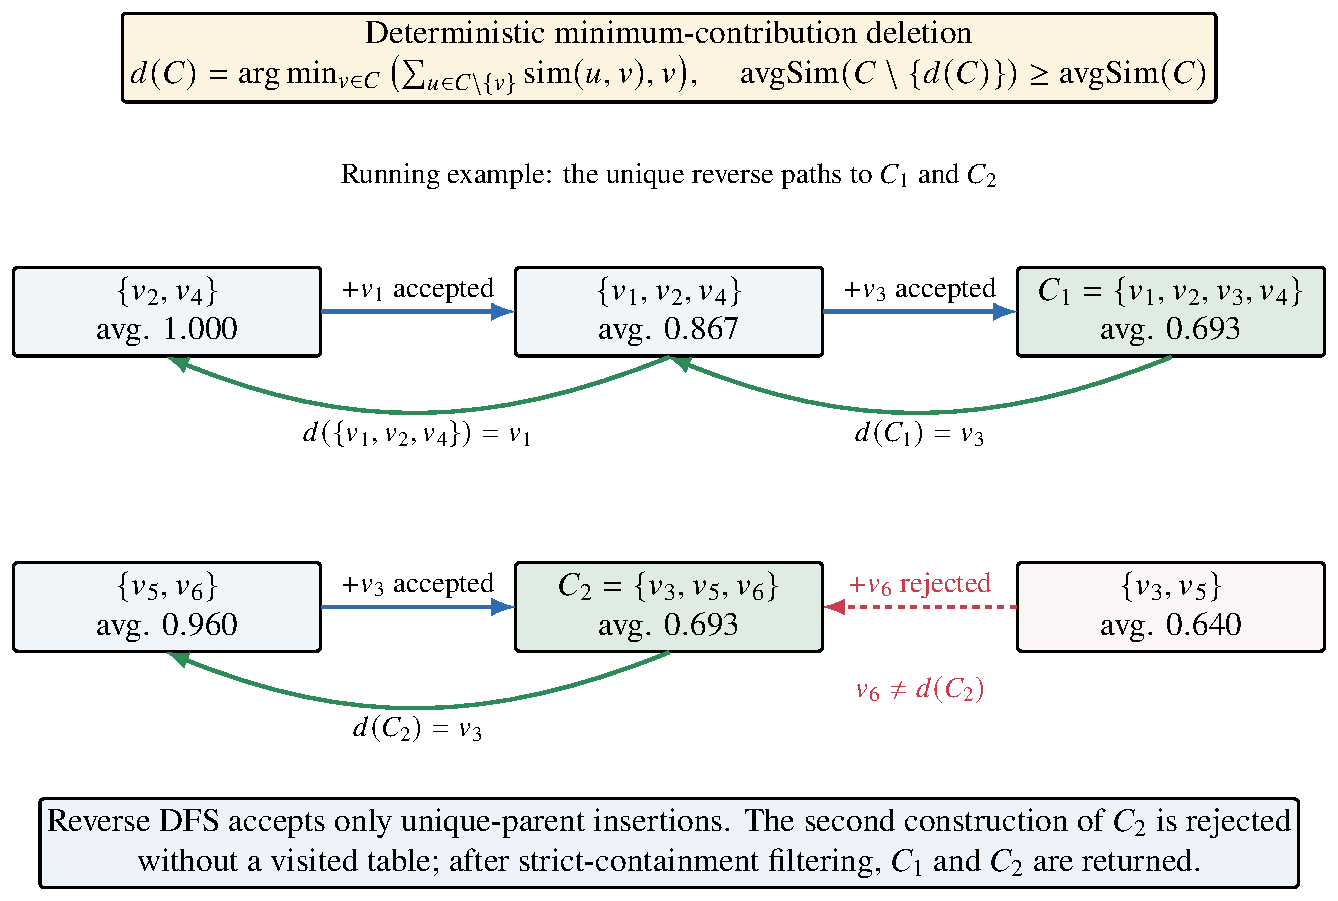
\includegraphics[width=0.8\linewidth]{tex-data/fig/monosem_workflow.pdf}
  \caption{Canonical ownership on the running example.}
  \Description{The canonical-parent rule, two accepted insertion paths in green, and a rejected duplicate construction of C2 in red.}
  \label{fig:monotone}
\end{figure}

\begin{algorithm}[t]
  \small
  \caption{\monoSemMCE: Canonical Reverse Search}
  \label{alg:monosem-mce}
  \SetKwFunction{FSearch}{Search}
  \SetKwProg{Fn}{Function}{:}{}
  \textbf{Input}: $G=(V,E)$, semantic vectors $\{x_v\}$, threshold $\tau$\\
  \textbf{Output}: All MSCs $\mathcal{R}$

  Precompute $\mathrm{sim}(u,v)$ for all $(u,v)\in E$\;
  $\mathcal{F} \leftarrow \emptyset$\;
  \For{each $(u,v)\in E$ with $u<v$ and $\mathrm{sim}(u,v)\geq\tau$
       \textbf{in parallel}}{
    $C\leftarrow\{u,v\}$; $S\leftarrow\mathrm{sim}(u,v)$\;
    $P\leftarrow N(u)\cap N(v)$\;
    $\acc[w]\leftarrow\mathrm{sim}(w,u)+\mathrm{sim}(w,v)$ for $w\in P$\;
    $a_C(u)=a_C(v)\leftarrow\mathrm{sim}(u,v)$\;
    \FSearch{$C,S,P,\acc,a_C$}\;
  }
  Apply Algorithm~\ref{alg:strsub}'s grouped strict-containment filter to $\mathcal{F}$, obtaining $\mathcal{R}$\;
  \Return $\mathcal{R}$\;
  \BlankLine
  \Fn{\FSearch{$C,S,P,\acc,a_C$}}{
    $k\leftarrow|C|$; $W\leftarrow S-\tau\binom{k}{2}$\;
    $\textit{hasValid}\leftarrow\textbf{false}$\;
    \For{each $v\in P$}{
      $\delta\leftarrow\acc[v]$\;
      \lIf{$W+\delta-\tau k<0$}{\textbf{continue}}
      $\textit{hasValid}\leftarrow\textbf{true}$\;
      $D\leftarrow C\cup\{v\}$\;
      Update $a_D$ from $a_C$ and $\mathrm{sim}(v,u)$ for $u\in C$\;
      \lIf{$v\neq\arg\min_{x\in D}(a_D(x),x)$}{\textbf{continue}}
      $P'\leftarrow P\cap N(v)$\;
      $\acc'[w]\leftarrow\acc[w]+\mathrm{sim}(w,v)$ for $w\in P'$\;
      \FSearch{$D,S+\delta,P',\acc',a_D$}\;
    }
    \lIf{\textbf{not} $\textit{hasValid}$}{$\mathcal{F}\leftarrow\mathcal{F}\cup\{C\}$}
  }
\end{algorithm}
\stitle{Feasible Edge Roots.}
Every feasible clique of size at least two reaches a feasible edge under
the deterministic deletion rule, so Algorithm~\ref{alg:monosem-mce} starts one tree
for each edge with similarity at least $\tau$.  A state stores the clique
$C$, its pairwise sum $S$, the common-neighbor set $P$, candidate
accumulators $\acc$, and the member contributions $a_C$.  No BK exclusion set
is required: uniqueness follows from the canonical-parent test rather
than from an insertion order.

\stitle{Surplus and Canonical-Child Tests.}
For $k=|C|$ and $\delta=\acc[v]$, the extension satisfies
\[
  \W(C\cup\{v\})=\W(C)+\delta-\tau k.
\]
If this value is negative, the child itself is infeasible and cannot lie
on the canonical path of any feasible answer, so it is safely skipped.
For a feasible child $D=C\cup\{v\}$, the algorithm updates every member's
similarity contribution and accepts $D$ only if $v=d(D)$.  Equivalently, the canonical
parent of $D$ must be exactly $C$.  This test removes alternative
insertion paths before recursion rather than after state materialization.
The flag $\mathit{hasValid}$ is set before the ownership test because it records
the existence of any feasible one-vertex extension, not the existence of an
owned child. A state with such an extension cannot itself be inclusion-wise
maximal; the extension is generated from its unique canonical parent.

The path property is used to assign unique parent ownership rather than to
order candidates.  The algorithm tests child feasibility directly and then
applies the minimum-contribution deletion rule.  This removes duplicate paths
before recursion without a candidate-order cutoff.  Accumulator values are
restored from saved values when backtracking, so the result does not depend on
reversing a sequence of floating-point additions.

\stitle{Inclusion-Wise Maximality.}
A state with no feasible single-vertex extension is added to
$\mathcal{F}$, but is not yet declared an MSC.  If such a candidate
$C$ is not inclusion-wise maximal, the finite family of feasible clique
supersets of $C$ contains an inclusion-wise maximal member $M$.  The
canonical search enumerates $M$ exactly once, and $M$ has no feasible
single extension, so it also belongs to $\mathcal{F}$.  The final
  grouped inverted-index containment filter consequently removes $C$.  Conversely,
an MSC is not contained in any other feasible candidate and is retained.

\begin{theorem}[Enumeration Correctness]
\label{thm:monosem-correctness}
Algorithm~\ref{alg:monosem-mce} generates every $\tau$-semantic clique
of size at least two exactly once and returns exactly all MSCs.
\end{theorem}
\begin{proof}
Existence follows by reversing the repeated deterministic deletions in
Theorem~\ref{thm:monotone}; every prefix is feasible and therefore passes
the surplus test.  Uniqueness follows because every non-root feasible
clique has the single parent $C\setminus\{d(C)\}$, and only that parent
accepts it as a child.  The preceding containment argument proves that
the final filter retains precisely the inclusion-wise maximal feasible
cliques.
\end{proof}


\stitle{Complexity.}
\begin{theorem}[Time and Space Complexity of \monoSemMCE]
  \label{thm:monosem-complexity}
  Let $F_\tau$ be the number of feasible cliques of size at least two, $K$ the
  maximum clique size, $\Delta$ the maximum degree, $T$ the number of workers,
  and $N=|\mathcal F|$ the number of terminal candidates.  A conservative
  bound for canonical search is
  \[
    O\!\left(F_\tau\Delta(\Delta+K)\log\Delta
      +KN\log N+K\sum_{S\in\mathcal F}L_{\min}(S)\right),
  \]
  with $O(m+T(n+K\Delta)+NK)$ words of space in addition to vector storage.
\end{theorem}
\begin{proof}
  Canonical ownership bounds accepted states by $F_\tau$.  A state tests at
  most $\Delta$ candidates.  For each candidate, common-neighbor intersection
  and accumulator maintenance cost $O(\Delta)$ conservatively, while updating
  and comparing at most $K$ member contributions uses cached similarities with
  $O(\log\Delta)$ lookup.  This is bounded by
  $O(\Delta(\Delta+K)\log\Delta)$ per accepted state.  The final filter has the
  same $O(KN\log N+K\sum_S L_{\min}(S))$ cost as in \subEnum.

  Sparse similarity adjacency and neighbor bitmaps use $O(m)$ words.  Each
  worker owns an $O(n)$ generation-tagged accumulator and $O(K\Delta)$ DFS
  scratch space.  Terminal candidates occupy $O(NK)$ words; no feasible-size
  layer or visited-state table is materialized.
\end{proof}

\noindent\textbf{Remark.}
Increasing $\tau$ contracts the feasible-state family $F_\tau$, which gives
\monoSemMCE\ its selective-threshold operating region.  \subEnum\ instead pays
the structural MCE cost and is less sensitive to $F_\tau$.
\section{Implementation Optimizations}
\label{sec:opt}

The following optimizations are applied to \monoSemMCE\ and \subEnum\
without affecting correctness.  They address three categories of
bottlenecks: parallel load balance, repeated computation in the
expansion inner loop, and memory access cost for neighbor intersection
and similarity lookup.

\stitle{Parallel Decomposition and Load Balance.}
\subEnum\ Phase~1 parallelizes BK over seed vertices under degeneracy
ordering: each seed $v$ spawns an independent subproblem over its
forward neighborhood $(P_v, X_v)$, and distinct seeds share no mutable
state and require no synchronization. Phase~2 normally processes each
structural maximal clique with thread-local candidate lists, but a few large
host cliques can dominate this work. For such a clique, each fixed-cardinality
layer is partitioned by its smallest selected vertex. These partitions are
disjoint and may run concurrently because distinct equal-size subsets cannot
strictly contain one another. A barrier merges the feasible subsets before the
next smaller layer, preserving all local-containment decisions while exposing
parallelism inside a single expensive host clique. Thread-local candidates are
merged only after processing, avoiding lock contention on the output.

\monoSemMCE\ assigns each feasible edge root to one canonical tree.
Distinct trees contain disjoint feasible-clique states, so roots are
dispatched with dynamic OpenMP scheduling and require no shared visited
table.  Each worker performs DFS with thread-local accumulators, scratch
buffers, statistics, and candidate output; only the final merge and
  containment filter synchronize globally.

\stitle{Incremental Candidate Maintenance.}
When expanding state $(C, \simsum, P, \acc)$ by vertex $v$, the child
state requires an updated candidate set $P' = P \cap N(v)$ and an
updated accumulator $\acc'$.  A na\"{i}ve implementation recomputes
$\acc'$ from scratch at cost $O(|P'| \cdot |C|)$ per expansion.

Since $\acc[w] = \sum_{u \in C} \mathrm{sim}(w, u)$, the child
accumulator satisfies
\[
  \acc'[w] = \acc[w] + \mathrm{sim}(w, v) \quad \forall\, w \in P',
\]
reducing the update to $O(|P'|)$ regardless of clique depth.
The DFS records each previous accumulator value and restores it exactly
after the recursive call.  Reversing an update by subtracting the same
floating-point similarity is not equivalent: rounding can accumulate
across sibling branches and change a threshold decision.  Candidate
ordering has no correctness role in canonical search, so the standard
implementation performs no per-state sort.

\stitle{Sparse Blocked Bitmap for Neighbor Intersection.}
Candidate set intersection $P' = P \cap N(v)$ is the innermost
operation of every expansion.  We represent each adjacency list as a
\emph{sparse blocked bitmap}: vertices are indexed by
$\lfloor v/64 \rfloor$, and only non-empty 64-bit blocks are stored as
(index, word) pairs in sorted order.  Intersection of two rows
executes a merge-style scan over their block lists, applying bitwise
AND only to matching block indices and extracting set bits via
\texttt{ctz}.  The cost is $O(b_u + b_v)$ where $b_u, b_v$ count
non-empty blocks in each row, compared to $O(n/64)$ for a dense
bitmap.

This advantage compounds with search depth: at layer $\ell$, every
candidate $w \in P$ is a common neighbor of all $\ell{+}2$ clique
members, so $|P|$ decreases with $\ell$ and each row's active block
count shrinks accordingly.  The per-intersection cost therefore
decreases with depth.

\stitle{Similarity Computation with Reorder-Aware Caching.}
All pairwise similarities are precomputed once and stored in sorted
adjacency lists for $O(\log \deg(u))$ lookup via binary search.
Inner products use 8-wide AVX2 SIMD over the float32 vector store.  Edge
similarities remain float32 to control memory traffic, while similarity
sums, per-candidate accumulators, surpluses, and threshold products are
maintained in double precision.  Every feasibility test compares these
double-precision quantities directly with an inclusive boundary; no
algorithm-specific epsilon is used.

To reduce cache miss cost on repeated lookups, vertices are reordered
by a degree-descending BFS before vectors are stored contiguously in
memory.  A vertex $u$ with degree $d_u$ participates in $O(d_u)$
expansions as a candidate across the search; placing high-degree
vertices at low memory offsets concentrates the most frequently
accessed vectors into a small number of cache lines, reducing cold
misses on the hot working set.
\section{Experiments}
\label{sec:exp}

We organize the evaluation around five research questions. RQ1 evaluates exact
end-to-end performance; RQ2 identifies threshold and scale regimes; RQ3
isolates parallel and pruning mechanisms; RQ4 measures how the MSC output space
changes with $\tau$; and RQ5 examines semantic quality against structurally
defined alternatives.

\subsection{Experimental Setup}
\label{sec:exp-setup}

\stitle{Methods and comparison scope.}
\StructBK\ is a Tomita-pivot structural MCE implementation and supplies only a
threshold-independent structural-time reference. \semBK\ is the exact direct
baseline: it uses the same MSC definition, threshold, similarity values, and
strict-containment filter as \subEnum\ and \monoSemMCE. Consequently, runtime
speedups are claimed only among these three exact MSC methods. \pairSim\ keeps edges whose endpoint similarity reaches $\tau$ and then runs
structural MCE. FastQC enumerates maximal quasi-cliques under a degree-density
constraint~\cite{yu2023fastqc}, while FaPlex enumerates maximal $2$-plexes that
may omit one incident edge per vertex~\cite{zhou2020faplex}. These methods
define different pattern families and are used only for output-quality
comparisons.
\stitle{Datasets.}
The common grid contains three graphs with natural attributes and five public
graphs with reproducibly generated attributes. FB15K-237 descriptions use
all-MiniLM-L6-v2 embeddings; GitHub-Social uses its official 4,005-dimensional
developer features; and ogbn-arxiv retains its official 128-dimensional node
features~\cite{toutanova2015observed,wang2020ogb}. For email-Enron and the four
SuiteSparse graphs~\cite{leskovec2014snap,davis2011uf}, PCG64 draws 256
coordinates independently from $U[-1,1)$ under fixed dataset seeds, followed
by $\ell_2$ normalization. Graph structure is never synthesized.

\begin{table}[t]
\footnotesize
\centering
\setlength{\tabcolsep}{3.6pt}
\begin{tabular*}{\linewidth}{@{\extracolsep{\fill}}lrrrl@{}}
\toprule
Dataset & $|V|$ & $|E|$ & $D$ & Attributes \\
\midrule
FB15K-237 & 14,541 & 248,611 & 384 & natural \\
GitHub-Social & 37,700 & 289,003 & 4,005 & natural \\
ogbn-arxiv & 169,343 & 1,157,799 & 128 & natural \\
email-Enron & 36,692 & 183,831 & 256 & generated \\
sc-nasasrb & 54,870 & 1,311,227 & 256 & generated \\
sc-pkustk11 & 87,804 & 2,565,054 & 256 & generated \\
sc-pwtk & 217,891 & 5,653,221 & 256 & generated \\
sc-ldoor & 909,537 & 20,770,807 & 256 & generated \\
\bottomrule
\end{tabular*}
\caption{[RQ1--RQ5] Eight public graphs cover natural and controlled vector attributes.}
\label{tab:datasets}
\end{table}

\stitle{Protocol.}
Experiments run on an AMD Ryzen~9 7945HX workstation with 16 physical cores,
32 hardware threads, and 32\,GiB memory under Windows~11 and MSYS2 GCC~13.2.
Each process is limited to 16\,GiB and 32 OpenMP threads. The uniform timeout is
1,200 seconds. Completed runtime configurations are repeated three times and
reported by the median; a timeout is recorded after one complete limit window.
Runtime binaries contain no statistics counters.

Absolute cosine values are not comparable across vector sources. We therefore
derive thresholds from the edge-similarity distribution of each dataset. The
common grid fixes $q_{20}$, $q_{80}$, and $q_{99}$ before execution; sensitivity
experiments use $q_{5}$, $q_{20}$, $q_{50}$, $q_{70}$, $q_{80}$, $q_{90}$,
$q_{95}$, $q_{97}$, and $q_{99}$. All exact methods receive the same stored
float32 edge similarities and evaluate inclusive feasibility using
double-precision sums.

\subsection{RQ1: Exactness and End-to-End Efficiency}
This experiment answers RQ1 by comparing complete MSC output sets and total
runtime under the common grid. Exhaustive oracles first test 225,000
vertex-bound instances and 40,001 canonical-parent instances, including
negative similarities, equality at $\tau$, and tied minimum contributions.
On real graphs, jointly completed methods agree on normalized clique sets,
counts, and size histograms. In particular, all three exact methods return
263,721, 71,118, and 2,636 MSCs on GitHub-Social at $q_{20}$, $q_{80}$, and
$q_{99}$, respectively; \subEnum\ and \monoSemMCE\ also agree on every jointly
completed row of Table~\ref{tab:main-runtime}.

\begin{table*}[t]
\scriptsize
\centering
\setlength{\tabcolsep}{2.5pt}
\renewcommand{\arraystretch}{1.02}
\begin{tabular*}{0.98\textwidth}{@{\extracolsep{\fill}}lcrrrrr@{}}
\toprule
Dataset & $q$ & MSCs & \shortstack{\StructBK\\structure} & \semBK & \subEnum & \monoSemMCE \\
\midrule
FB15K-237 & 20 & 206,470 & \multirow{3}{*}{\cellcolor{gray!12}0.103} & TLE & \cellcolor{bestgreen}\textbf{0.221} & TLE \\
 & 80 & 76,106 & & TLE & \cellcolor{bestgreen}\textbf{9.132} & TLE \\
 & 99 & 7,476 & & TLE & 45.234 & \cellcolor{bestgreen}\textbf{10.091} \\
\midrule
GitHub-Social & 20 & 263,721 & \multirow{3}{*}{\cellcolor{gray!12}0.110} & 55.269 & \cellcolor{bestgreen}\textbf{0.327} & 29.315 \\
 & 80 & 71,118 & & 44.161 & \cellcolor{bestgreen}\textbf{0.314} & 20.551 \\
 & 99 & 2,636 & & 38.213 & 0.391 & \cellcolor{bestgreen}\textbf{0.118} \\
\midrule
ogbn-arxiv & 20 & 925,239 & \multirow{3}{*}{\cellcolor{gray!12}0.309} & 2.783 & \cellcolor{bestgreen}\textbf{1.233} & 3.357 \\
 & 80 & 226,936 & & 1.206 & \cellcolor{bestgreen}\textbf{0.872} & 1.610 \\
 & 99 & 10,261 & & 1.318 & 0.843 & \cellcolor{bestgreen}\textbf{0.197} \\
\midrule
email-Enron & 20 & 223,703 & \multirow{3}{*}{\cellcolor{gray!12}0.090} & 18.330 & \cellcolor{bestgreen}\textbf{0.259} & 16.739 \\
 & 80 & 60,352 & & 21.369 & 1.266 & \cellcolor{bestgreen}\textbf{0.083} \\
 & 99 & 1,819 & & 9.608 & 0.206 & \cellcolor{bestgreen}\textbf{0.033} \\
\midrule
sc-nasasrb & 20 & 28,154 & \multirow{3}{*}{\cellcolor{gray!12}0.090} & TLE & \cellcolor{bestgreen}\textbf{0.301} & TLE \\
 & 80 & 834,914 & & TLE & 102.820 & \cellcolor{bestgreen}\textbf{0.759} \\
 & 99 & 12,742 & & TLE & 0.415 & \cellcolor{bestgreen}\textbf{0.079} \\
\midrule
sc-pkustk11 & 20 & 22,612 & \multirow{3}{*}{\cellcolor{gray!12}0.143} & TLE & \cellcolor{bestgreen}\textbf{0.645} & TLE \\
 & 80 & 2,214,411 & & TLE & TLE & \cellcolor{bestgreen}\textbf{2.219} \\
 & 99 & 24,891 & & TLE & 0.611 & \cellcolor{bestgreen}\textbf{0.167} \\
\midrule
sc-pwtk & 20 & 58,523 & \multirow{3}{*}{\cellcolor{gray!12}0.286} & TLE & \cellcolor{bestgreen}\textbf{1.093} & TLE \\
 & 80 & 4,483,887 & & TLE & TLE & \cellcolor{bestgreen}\textbf{3.977} \\
 & 99 & 54,907 & & TLE & 1.364 & \cellcolor{bestgreen}\textbf{0.421} \\
\midrule
sc-ldoor & 20 & 274,585 & \multirow{3}{*}{\cellcolor{gray!12}1.679} & TLE & \cellcolor{bestgreen}\textbf{4.870} & TLE \\
 & 80 & 13,473,317 & & TLE & 563.996 & \cellcolor{bestgreen}\textbf{14.944} \\
 & 99 & 202,030 & & TLE & 4.845 & \cellcolor{bestgreen}\textbf{1.658} \\
\bottomrule
\end{tabular*}
\caption{[RQ1] Median end-to-end seconds; the two specialized methods jointly complete all 24 MSC workloads.}
\label{tab:main-runtime}
\end{table*}

Table~\ref{tab:main-runtime} shows that \subEnum\ completes 22 of 24 workloads
and every $q_{20}$ row, while \monoSemMCE\ resolves the two intermediate rows
where host-clique subset enumeration reaches TLE. At $q_{99}$, canonical search
is faster on all eight graphs, with speedups from $2.92\times$ on sc-ldoor to
$6.24\times$ on email-Enron. \semBK\ completes all nine natural-attribute rows
except FB15K-237, but its pivot-free search is slower than the best specialized
method on every completed row. The gray \StructBK\ column is reported only to
separate structural enumeration cost from semantic processing.

\subsection{RQ2: Threshold and Scale Regimes}
This experiment answers RQ2 by varying selectivity independently of graph size.
Figure~\ref{fig:threshold-runtime} uses the full fixed quantile grid. On
ogbn-arxiv, both specialized methods complete the sweep and cross near
$q_{95}$; on sc-ldoor, \subEnum\ covers low and intermediate thresholds, while
\monoSemMCE\ becomes dominant once the feasible canonical tree contracts.
TLE points are shown at the fixed limit and are not interpolated.

\begin{figure}[t]
\centering

\includegraphics[width=0.72\linewidth]{tex-data/fig/threshold_runtime_legend.pdf}
\begin{subfigure}[t]{0.495\linewidth}
\centering
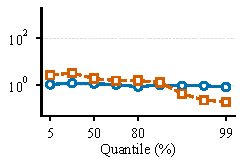
\includegraphics[width=\linewidth]{tex-data/fig/threshold_runtime_arxiv.pdf}
\caption{ogbn-arxiv}
\end{subfigure}\hfill
\begin{subfigure}[t]{0.495\linewidth}
\centering
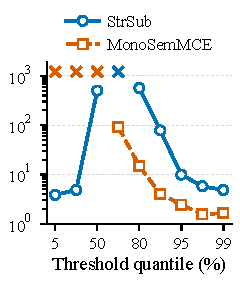
\includegraphics[width=\linewidth]{tex-data/fig/threshold_runtime_ldoor.pdf}
\caption{sc-ldoor}
\end{subfigure}
\caption{[RQ2] Threshold sweeps reveal complementary runtime regimes.}
\Description{Runtime over nine fixed threshold quantiles on ogbn-arxiv and sc-ldoor.}
\label{fig:threshold-runtime}
\end{figure}

Figure~\ref{fig:scale-regime} repeats the comparison on nested induced
ogbn-arxiv graphs whose vertices follow one fixed degree order. The crossover
remains at $q_{95}$ from 25K vertices through the full graph. At $q_{99}$ on
the full graph, \subEnum\ and \monoSemMCE\ take 0.707 and 0.200 seconds and
return the same 10,261 MSCs. The stable boundary links the regime change to
semantic selectivity rather than one graph size.

\begin{figure}[t]
\centering
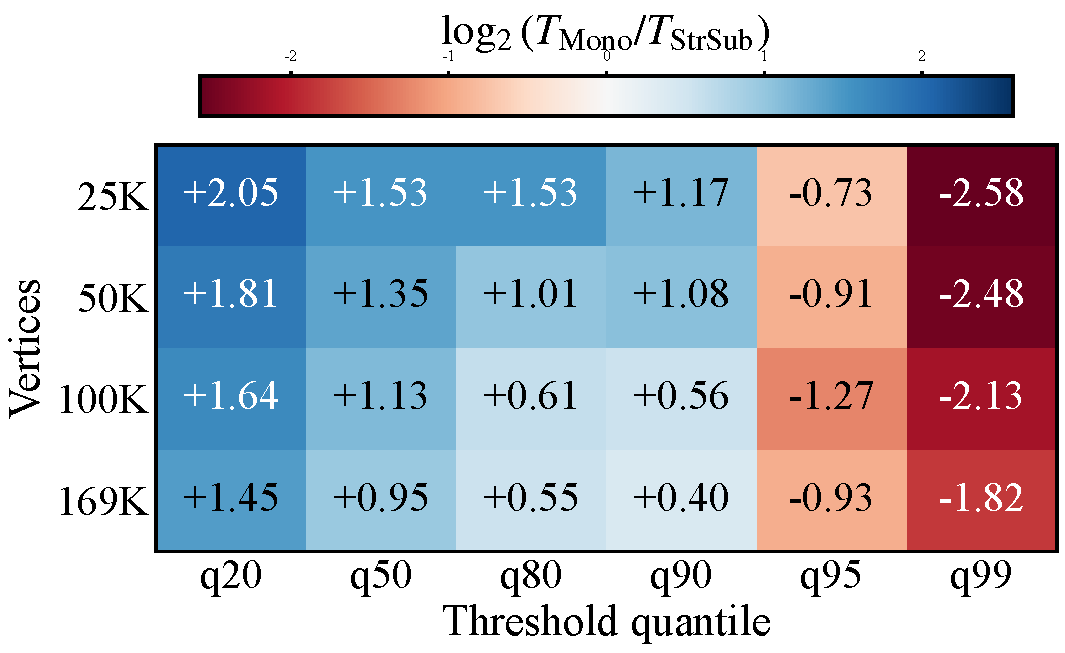
\includegraphics[width=0.80\linewidth]{tex-data/fig/scale_regime.pdf}
\caption{[RQ2] The \monoSemMCE\ high-threshold region persists across four nested graph sizes.}
\Description{Runtime ratio between StrSub and MonoSemMCE over graph sizes and threshold quantiles.}
\label{fig:scale-regime}
\end{figure}

\subsection{RQ3: Parallelism and Search Mechanisms}
This experiment answers RQ3 by connecting parallel speedup to measured search
work. Figure~\ref{fig:parallel-scaling} reports one representative workload for
each specialized algorithm. Dynamic edge-root scheduling gives \monoSemMCE\
$5.62\times$ speedup at 32 threads. Fixed-size subset partitioning gives
\subEnum\ $2.39\times$ at 16 threads and $2.26\times$ at 32 threads. Separately
collected phase counters attribute 98.88\% of its 32-thread work to host-clique
subset processing, while the final global filter takes 65 ms; the remaining
saturation is therefore caused by unequal host-clique tasks.

\begin{figure}[t]
\centering
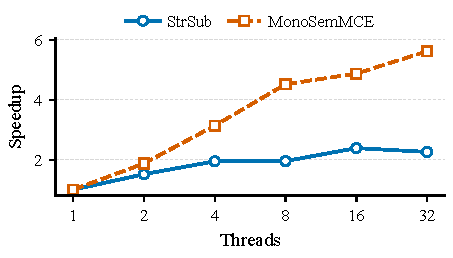
\includegraphics[width=0.80\linewidth]{tex-data/fig/parallel_scaling.pdf}
\caption{[RQ3] Independent root scheduling yields parallel gains for both specialized searches.}
\Description{Speedup from one to 32 threads for representative StrSub and MonoSemMCE workloads.}
\label{fig:parallel-scaling}
\end{figure}

Figure~\ref{fig:mechanisms} relates runtime regimes to work counters collected
outside timing runs. On sc-nasasrb at $q_{99}$, Top-Edge pruning reduces subset
tests from 16.50 to 12.95 million, and the vertex bound reduces them from 80.28
to 12.95 million. On ogbn-arxiv, accepted canonical states contract from 17.08
million at $q_5$ to 18,011 at $q_{99}$.

\begin{figure}[t]
\centering
\begin{subfigure}[t]{0.495\linewidth}
\centering
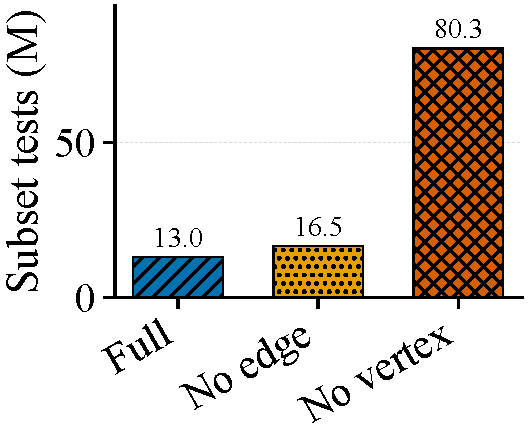
\includegraphics[width=\linewidth]{tex-data/fig/mechanism_strsub.pdf}
\caption{\subEnum\ pruning}
\end{subfigure}\hfill
\begin{subfigure}[t]{0.495\linewidth}
\centering
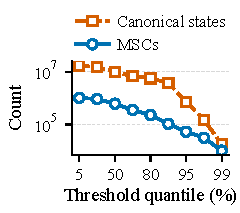
\includegraphics[width=\linewidth]{tex-data/fig/mechanism_monosem.pdf}
\caption{\monoSemMCE\ states}
\end{subfigure}
\caption{[RQ3] Search bounds and canonical contraction reduce explored states.}
\Description{Subset tests by StrSub variant and accepted MonoSemMCE states by threshold.}
\label{fig:mechanisms}
\end{figure}

\begin{table}[t]
\footnotesize
\centering
\setlength{\tabcolsep}{4.0pt}
\begin{tabular*}{\linewidth}{@{\extracolsep{\fill}}llrr@{}}
\toprule
Component & Metric / workload & Full & Removed \\
\midrule
Top-Edge & tests (M) / nasa $q_{99}$ & \cellcolor{bestgreen}\textbf{12.95} & 16.50 \\
Vertex bound & tests (M) / nasa $q_{99}$ & \cellcolor{bestgreen}\textbf{12.95} & 80.28 \\
Local containment & GiB / FB15K $q_{80}$ & \cellcolor{bestgreen}\textbf{0.12} & 2.26 \\
\bottomrule
\end{tabular*}
\caption{[RQ3] Exact \subEnum\ ablations reduce subset work or candidate memory without changing outputs.}
\label{tab:ablation}
\end{table}

The corresponding runtimes are 0.287 versus 0.324 seconds for Top-Edge,
0.287 versus 0.312 seconds for the vertex bound, and 8.060 versus 11.685
seconds for local containment. Table~\ref{tab:generation-ablation} then holds
the feasibility test, similarity cache, and final filter fixed while replacing
only duplicate-state organization. Canonical ownership is fastest and uses the
least memory on both workloads; every variant returns the same normalized MSC
set and size histogram.

\begin{table}[t]
\footnotesize
\centering
\setlength{\tabcolsep}{4.0pt}
\begin{tabular*}{\linewidth}{@{\extracolsep{\fill}}lrrrr@{}}
\toprule
& \multicolumn{2}{c}{ogbn $q_{95}$} & \multicolumn{2}{c}{nasa $q_{80}$} \\
\cmidrule(lr){2-3}\cmidrule(lr){4-5}
Generation & s & GiB & s & GiB \\
\midrule
\rowcolor{bestgreen}Canonical & \textbf{0.388} & \textbf{0.39} & \textbf{0.729} & \textbf{0.22} \\
Visited DFS & 2.432 & 0.53 & 3.069 & 0.64 \\
Layered & 1.635 & 0.49 & 3.922 & 0.81 \\
\bottomrule
\end{tabular*}
\caption{[RQ3] Canonical ownership improves both runtime and memory over visited and layered generation.}
\label{tab:generation-ablation}
\end{table}

\subsection{RQ4: MSC Output Space}
This experiment answers RQ4 by measuring exact output counts and mean sizes on
FB15K-237, ogbn-arxiv, sc-nasasrb, and sc-ldoor over
$q_{20},q_{50},q_{80},q_{95},q_{99}$. Figure~\ref{fig:result-distribution}
normalizes each value by \StructBK\ on the same graph. The geometric-mean count
ratios are 1.04, 7.50, 3.53, 0.61, and 0.11: intermediate thresholds split
large structural cliques into many feasible subsets that are maximal by
inclusion. Selective thresholds instead contract the result family. Mean size decreases
from 1.06 to 0.39 of the structural reference over the same grid.

\begin{figure}[t]
\centering
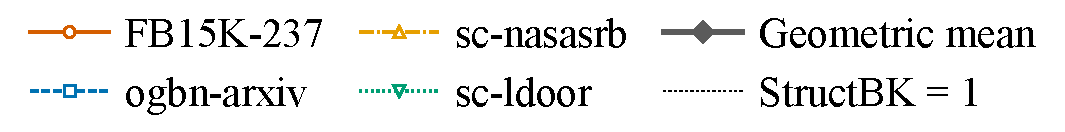
\includegraphics[width=0.94\linewidth]{tex-data/fig/result_distribution_legend.pdf}
\begin{subfigure}[t]{0.495\linewidth}
\centering
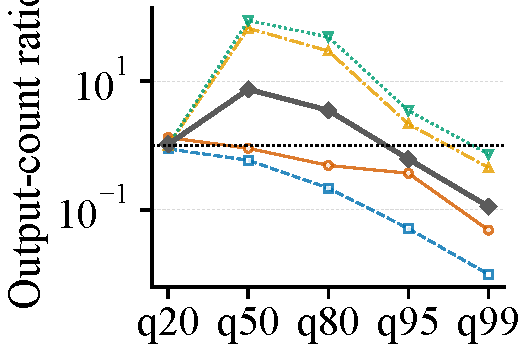
\includegraphics[width=\linewidth]{tex-data/fig/result_distribution_count.pdf}
\caption{Output count}
\end{subfigure}\hfill
\begin{subfigure}[t]{0.495\linewidth}
\centering
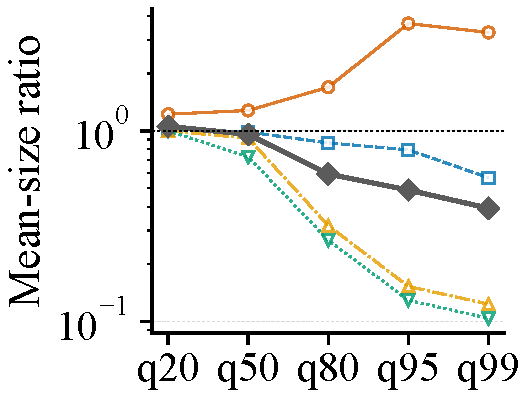
\includegraphics[width=\linewidth]{tex-data/fig/result_distribution_size.pdf}
\caption{Mean size}
\end{subfigure}
\caption{[RQ4] MSCs expand at intermediate thresholds and contract sharply in the selective regime.}
\Description{Normalized MSC count and mean size over five threshold quantiles on four datasets.}
\label{fig:result-distribution}
\end{figure}

\subsection{RQ5: Group Preservation and External Pattern Families}
RQ5 separates a definition comparison from a cross-model comparison. For the
definition comparison, the reference cover consists of all MSCs of size at
least ten at $q_{80}$ on GitHub-Social and ogbn-arxiv-25K. The response cover
contains every non-singleton \pairSim\ output at the same $\tau$; retaining
small response groups avoids attributing losses to a reporting cutoff.
Because both covers overlap, we use Extended B$^3$ Recall
\cite{amigo2009bcubed}, whose cluster-completeness property penalizes members
of one reference group being separated across response groups. We also report
the standard best-match community recall
\cite{yang2013bigclam,hric2014recovery}
\[
  R_{\max}(C)=\max_{P\in\mathcal P}\frac{|C\cap P|}{|C|},
\]
which has the direct interpretation that one PairSim output can retain at most
this fraction of MSC $C$.

Figure~\ref{fig:definition-recovery} shows a pronounced definition effect.
On GitHub-Social, \pairSim\ attains B$^3$ Recall 0.156 and mean best-match
recall 0.450; none of the 605 reference MSCs is retained intact. On
ogbn-arxiv-25K, the corresponding scores are 0.544 and 0.680, and only 0.32\%
of 624 reference MSCs are retained intact. The CDF gives the group-level
effect: every GitHub-Social MSC and 84.9\% of ogbn-arxiv-25K MSCs lose at
least 20\% of their members in the best matching \pairSim\ output. Thus the
every-pair constraint fragments groups that remain structurally complete and
collectively feasible under the same threshold.

\begin{figure}[t]
\centering

\includegraphics[width=0.94\linewidth]{tex-data/fig/definition_recovery_legend.pdf}
\vspace{-0.8ex}
\begin{subfigure}[t]{0.495\linewidth}
\centering
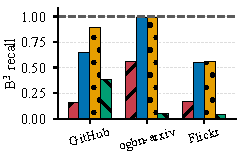
\includegraphics[width=\linewidth]{tex-data/fig/definition_recovery_summary.pdf}
\caption{Aggregate recovery}
\end{subfigure}\hfill
\begin{subfigure}[t]{0.495\linewidth}
\centering
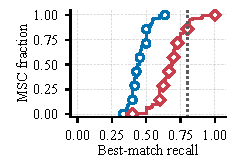
\includegraphics[width=\linewidth]{tex-data/fig/definition_recovery_cdf.pdf}
\caption{Per-group recovery}
\end{subfigure}
\caption{[RQ5] PairSim fragments collectively feasible complete groups.
Extended B$^3$ Recall evaluates the two overlapping covers; best-match recall
measures the largest fraction of each MSC retained by one PairSim output. The
MSC reference score is one by construction.}
\Description{The first panel compares Extended B-cubed and best-match recall
on two datasets. The second panel shows cumulative distributions of
best-match recall over reference MSCs.}
\label{fig:definition-recovery}
\end{figure}

For the external comparison, FastQC at $\gamma=0.9$ and FaPlex at $k=2$ are
evaluated together with \StructBK against the same size-ten MSC reference
cover; all result families use the fixed $q_{80}$ vectors and graph. We use
the symmetric best-match Average F1 established for overlapping community
covers \cite{yang2013bigclam}, and display its two directional components:
\emph{recovery} averages the best-match F1 from each MSC to the baseline
cover, whereas \emph{fidelity} averages the best-match F1 from each baseline
output to the MSC cover. The mean of these components is symmetric Average F1.
This separates recovery of MSCs from proliferation of additional baseline
patterns. The comparison measures agreement with the MSC target family, not
ground-truth clustering accuracy.

Figure~\ref{fig:external-quality} shows that recovery is high for all three
baselines, but fidelity is substantially lower. On GitHub-Social, the
recovery/fidelity pairs are 0.931/0.236 for \StructBK, 0.851/0.206 for FastQC,
and 0.865/0.123 for FaPlex. On ogbn-arxiv-25K they are 0.992/0.269,
0.898/0.208, and 0.907/0.181, respectively. High recovery is expected because
every MSC is a clique and therefore can be extended to a maximal clique,
quasi-clique, or 2-plex; fidelity exposes the extra result families created by
that extension. FastQC and FaPlex are not equivalent to \StructBK: their
pair-weighted edge densities are 0.942--0.952 rather than one, and fewer than
0.05\% of their retained outputs are complete cliques. They additionally cover
$12.5\times$--$27.6\times$ more vertices than MSC, with lower pairwise cosine.

\begin{figure}[t]
\centering
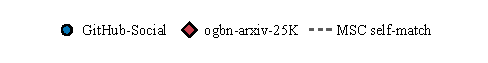
\includegraphics[width=0.94\linewidth]{tex-data/fig/external_recovery_legend.pdf}
\begin{subfigure}[t]{0.495\linewidth}
\centering
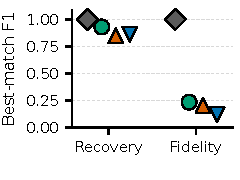
\includegraphics[width=\linewidth]{tex-data/fig/external_recovery_github.pdf}
\caption{GitHub-Social}
\end{subfigure}\hfill
\begin{subfigure}[t]{0.495\linewidth}
\centering
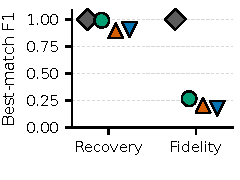
\includegraphics[width=\linewidth]{tex-data/fig/external_recovery_ogbn25k.pdf}
\caption{ogbn-arxiv-25K}
\end{subfigure}
\caption{[RQ5] Baselines recover most MSCs but produce many unmatched results.}
\Description{Two dot plots compare recovery and fidelity best-match F1 for
MSC, StructBK, FastQC, and FaPlex on two real graphs.}
\label{fig:external-quality}
\end{figure}
Figure~\ref{fig:quality-case} provides an instance-level explanation. The
largest label-pure MSC at ogbn-arxiv $q_{80}$ contains 18 papers from
\texttt{cs.IT} on private information retrieval. Its average similarity is
0.919 at $\tau=0.889$, although 20 of 153 pairs fall below $\tau$. Collective
coherence therefore preserves the complete research group that an every-edge
threshold separates.

\begin{figure}[t]
\centering
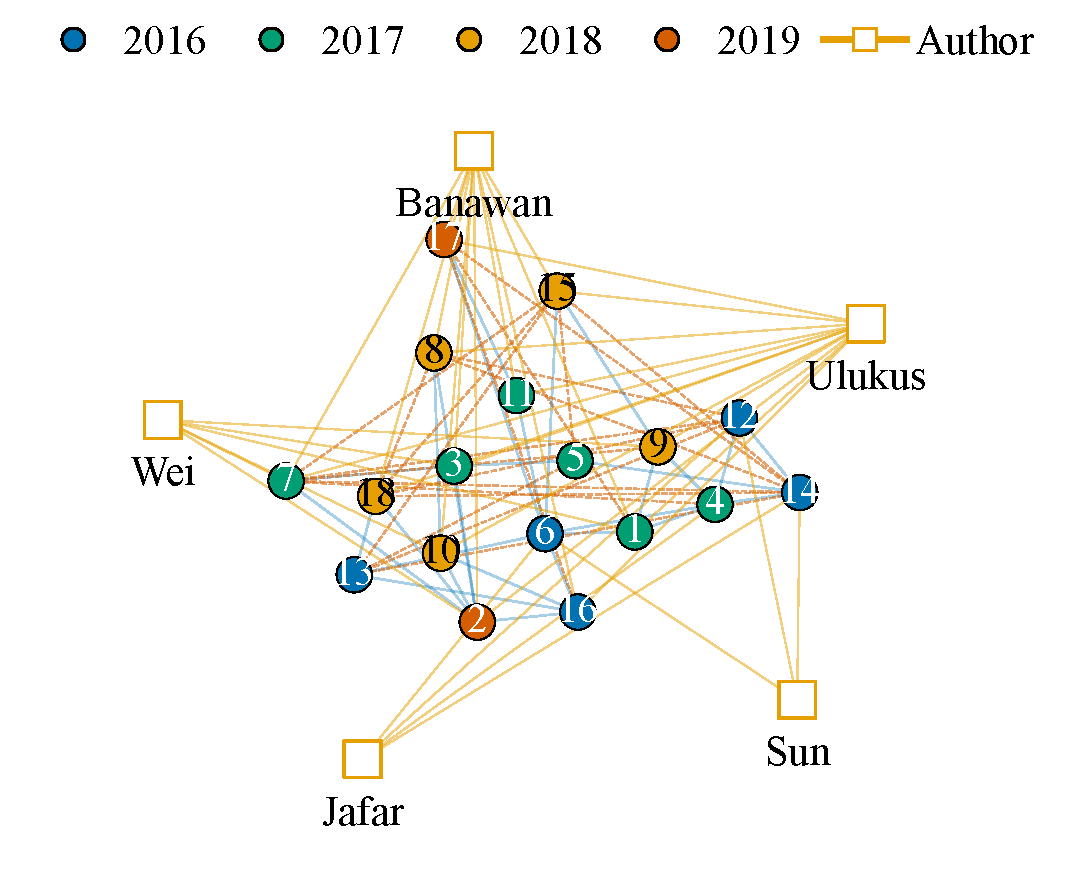
\includegraphics[width=0.80\linewidth]{tex-data/fig/quality_case_network.pdf}
\caption{[RQ5] An 18-paper MSC preserves a coherent research group despite 20 sub-threshold pairs.}
\Description{A paper network showing semantic-neighbor links and recurrent authors in one MSC.}
\label{fig:quality-case}
\end{figure}
\section{Related Work}
\label{sec:related}

\stitle{Clique Enumeration and Listing.}
Moon and Moser established the maximal-clique output bound~\cite{moon1965}.
BK backtracking~\cite{bron1973} and Tomita pivoting~\cite{tomita2006} form
the practical foundation, while degeneracy ordering targets sparse graphs
\cite{eppstein2010,eppstein2013}. Recent work improves branch selection
and termination for MCE~\cite{wang2025hbbmc}, develops edge-oriented
$k$-clique listing~\cite{wang2024kclique}, and summarizes large clique families
through comparison operators~\cite{li2025cliquecomparator}. These structural
techniques motivate the pivoted front end of \subEnum; MSC additionally couples
each search state to a non-monotone vector aggregate.

\stitle{Constrained Cohesive Subgraphs.}
Dense-subgraph models relax or augment the clique contract in different ways.
FastQC enumerates maximal quasi-cliques through co-designed pruning and
branching~\cite{yu2023fastqc}, while FaPlex enumerates maximal $k$-plexes with
a worst-case guarantee~\cite{zhou2020faplex}. Recent exact methods address
maximum $k$-plexes~\cite{gao2024kplex}, maximal biplexes~\cite{dai2024biplex},
fair cliques~\cite{zhang2025fairclique}, and similar-weight bicliques
~\cite{yang2025similarweight}. MSC retains structural completeness and constrains
the group-average vector similarity, so these models provide complementary
output families. Our exact efficiency baseline instead preserves the same MSC
contract throughout search.

\stitle{Attributed Community Search.}
Traditional attributed-graph methods combine topology and attributes under
different output contracts. CODICIL augments links with content similarity and
partitions the resulting graph~\cite{ruan2013codicil}, whereas ATC returns a
query-specific attribute-relevant truss community~\cite{huang2017}. Other
subgraph methods impose feature-subspace or correlation constraints
~\cite{moser2009,gunnemann2010,silva2012}. Recent systems transfer attributed
community search across graphs~\cite{fang2024iacs} or use pre-trained graph
transformers for unsupervised queries~\cite{wang2024transzero}. These methods
return a partition or one query-oriented community. MSC instead returns every
inclusion-wise maximal, structurally complete group whose collective vector
similarity reaches $\tau$.

\stitle{Vector Attributes.}
Vector-attributed graphs arise from knowledge-graph embeddings
\cite{bordes2013,sun2019}, random-walk representations
\cite{perozzi2014deepwalk}, and message-passing models
\cite{kipf2017}. Approximate vector indexes accelerate
unconstrained nearest-neighbor retrieval~\cite{malkov2020,johnson2021}. MSC evaluates similarities only on graph edges and preserves an
inclusive threshold exactly; our implementation therefore precomputes those
edge similarities and avoids approximation error inside enumeration.
\section{Conclusion}
\label{sec:conclusion}

We introduced maximal semantic clique (MSC) enumeration under an average pairwise similarity threshold, which identifies structurally complete cliques with guaranteed average pairwise semantic similarity. The problem generalizes classical MCE and is NP-complete. Its defining challenge is the non-monotonicity of the average-similarity constraint over the subset lattice, which invalidates the structural invariants that underpin the efficiency of standard Bron--Kerbosch algorithms.

We used \semBK\ as a direct pivot-free baseline and proposed two exact
algorithms with distinct operating regions. \subEnum\ decouples structural and semantic search,
restores the Tomita pivot in a $\tau$-agnostic structural phase, and applies
admissible edge and vertex-contribution bounds during exact subset enumeration.
\monoSemMCE\ is a high-$\tau$ specialization: the deterministic deletion rule
assigns each feasible clique one parent, so reverse DFS eliminates duplicate
insertion paths without visited sets or materialized layers. Both methods use
global strict-containment filtering to implement inclusion-wise maximality.

Exact-output tests validate the canonical search and every optional \subEnum\
component before timing.  On ogbn-arxiv, \subEnum\ is fastest at the
intermediate threshold, while \monoSemMCE\ is $4.28\times$ faster at
$q_{99}$; on FB15K-237, the corresponding high-threshold advantage is
$4.48\times$. Across the eight-dataset common grid, \subEnum\ completes 22 of
24 cells, and canonical search is $2.92\times$--$6.24\times$ faster on every
$q_{99}$ row. The controlled scale series places the crossover at $q_{95}$
across four graph sizes, while canonical edge-root scheduling reaches
$5.62\times$ speedup with 32 threads. Mechanism counters connect these results
to exact layer bounds in \subEnum\ and the rapid high-threshold contraction of
the canonical tree in \monoSemMCE. The fixed five-threshold output study also
captures the intermediate pattern-count expansion and high-threshold
contraction, while external labels and a real paper group establish the
semantic content of the returned MSCs. Future directions include stronger
admissible multi-step bounds, finer canonical-subtree scheduling, and
dynamic-graph extensions.
\bibliographystyle{ACM-Reference-Format}
\bibliography{references}

\end{document}
\endinput
